%============================================================================
% tento soubor pouzijte jako zaklad
% (c) 2008 Michal Bidlo
% E-mail: bidlom AT fit vutbr cz
%============================================================================
% kodovaní: iso-8859-2 (zmena prikazem iconv, recode nebo cstocs)
%----------------------------------------------------------------------------
% zpracování: make, make pdf, make desky, make clean
% připomínky posílejte na e-mail: bidlom AT fit.vutbr.cz
% vim: set syntax=tex encoding=latin2:
%============================================================================
\documentclass[cover]{fitthesis} % odevzdani do wisu - odkazy, na ktere se da klikat
%\documentclass[cover,print]{fitthesis} % pro tisk - na odkazy se neda klikat
%\documentclass[english,print]{fitthesis} % pro tisk - na odkazy se neda klikat
%      \documentclass[english]{fitthesis}
% * Je-li prace psana v anglickem jazyce, je zapotrebi u tridy pouzit 
%   parametr english nasledovne:
%      \documentclass[english]{fitthesis}
% * Neprejete-li si vysazet na prvni strane dokumentu desky, zruste 
%   parametr cover

% zde zvolime kodovani, ve kterem je napsan text prace
% "latin2" pro iso8859-2 nebo "cp1250" pro windows-1250, "utf8" pro "utf-8"
%\usepackage{ucs}
\usepackage[utf8]{inputenc}
\usepackage[T1]{fontenc}
\usepackage{url}
\usepackage{caption}
\usepackage{subcaption}
\usepackage{listings}
\usepackage{alltt}

\renewcommand{\ttdefault}{txtt}

\lstset{ %
  language=bash,                % the language of the code
  tabsize=2,                      % sets default tabsize to 2 spaces
  showspaces=false,               % show spaces adding particular underscores
  showstringspaces=false,         % underline spaces within strings
  showtabs=false,
  breaklines=true,                % sets automatic line breaking
  breakatwhitespace=false,        % sets if automatic breaks should only happen at whitespace
  basicstyle=\ttfamily,
  keywordstyle=\bfseries,
  identifierstyle=\ttfamily,
  commentstyle=\ttfamily,
  stringstyle=\ttfamily,
  showstringspaces=false
}

\DeclareUrlCommand\url{\def\UrlLeft{<}\def\UrlRight{>} \urlstyle{tt}}
\newcommand{\xen}{Xen\textsuperscript{\textregistered}\ }
\newcommand{\linux}{Linux\textsuperscript{\textregistered}}
\newcommand{\jdbc}{JDBC\textsuperscript{\texttrademark}}

%zde muzeme vlozit vlastni balicky


% =======================================================================
% balíček "hyperref" vytváří klikací odkazy v pdf, pokud tedy použijeme pdflatex
% problém je, že balíček hyperref musí být uveden jako poslední, takže nemůže
% být v šabloně
\ifWis
\ifx\pdfoutput\undefined % nejedeme pod pdflatexem
\else
  \usepackage{color,fancyvrb}
  \usepackage[unicode,colorlinks,hyperindex,plainpages=false,pdftex]{hyperref}
  \definecolor{links}{rgb}{0.4,0.5,0}
  \definecolor{anchors}{rgb}{1,0,0}
  \definecolor{gray}{rgb}{0.4,0.4,0.4}
  \definecolor{javared}{rgb}{0.6,0,0} % for strings
  \definecolor{javagreen}{rgb}{0.25,0.5,0.35} % comments
  \definecolor{javapurple}{rgb}{0.5,0,0.35} % keywords
  \definecolor{javadocblue}{rgb}{0.25,0.35,0.75} % javadoc
  \def\AnchorColor{anchors}
  \def\LinkColor{links}
  \def\pdfBorderAttrs{/Border [0 0 0] }  % bez okrajů kolem odkazů
  \pdfcompresslevel=9
  \lstset{language=Java,
      basicstyle=\ttfamily,
      keywordstyle=\color{javapurple}\bfseries,
      stringstyle=\color{javared},
      commentstyle=\color{javagreen},
      morecomment=[s][\color{javadocblue}]{/**}{*/},
      numbersep=10pt,
      tabsize=4,
      showspaces=false,
      showstringspaces=false
  }
\fi
\fi
\usepackage{cleveref}
\crefformat{footnote}{#2\footnotemark[#1]#3}
%Informace o praci/projektu
%---------------------------------------------------------------------------
\projectinfo{
  %Prace
  project=BP,            %typ prace BP/SP/DP/DR
  year=2012,             %rok
  date=\today,           %datum odevzdani
  %Nazev prace
  title.cs={Srovnání výkonu a vlastností objektově orientovaných databází},  %nazev prace v cestine
  title.en={Comparison of Properties and Performance of Object Oriented Databases}, %nazev prace v anglictine
  %Autor
  author={Daniel Kozák},   %jmeno prijmeni autora
  %author.title.p=Bc., %titul pred jmenem (nepovinne)
  %author.title.a=PhD, %titul za jmenem (nepovinne)
  %Ustav
  department=UIFS, % doplnte prislusnou zkratku: UPSY/UIFS/UITS/UPGM
  %Skolitel
  supervisor= Jan Zelený, %jmeno prijmeni skolitele
  supervisor.title.p=Ing.,   %titul pred jmenem (nepovinne)
  %supervisor.title.a=    %titul za jmenem (nepovinne)
  %Klicova slova, abstrakty, prohlaseni a podekovani je mozne definovat 
  %bud pomoci nasledujicich parametru nebo pomoci vyhrazenych maker (viz dale)
  %===========================================================================
  %Klicova slova
  keywords.cs={Databáze, databázové systémy, SŘBD, objektové databáze, relační databáze, objektově relační mapování, ORM, OHM, Java, NoSQL, reflexe, introspekce.}, %klicova slova v ceskem jazyce
  keywords.en={Database, Database systems, DBMS, object database, relational database, object-relational mapping, ORM, OHM, Java Language, NoSQL, reflection, introspection.}, %klicova slova v anglickem jazyce
  %Abstract
  abstract.cs={V této práci čtenáře seznámím se základními modely, jenž se používají pro ukládání dat v datbazových systémech. Dále čtenáři popíši způsoby ukládání objektů jazyka Java, kde mu nadále vysvětlím pojmy jako objektově relační mapování, reflexe a introspekce. Následně zde představím existující implementace, které se v jazyce Java používají pro ukládání objektových dat. Poté popíši metodiku pro testování výkonu jednotlivých řešení. Podle této metodiky provedu testování a nakonec zhodnotím získané výsledky.  
}, % abstrakt v ceskem jazyce
  abstract.en={In this thesis, the reader learns basic models, which are use for storing data in database systems. Next I describe a way, how to store objects in Java Language and explain expressions like object-relational mapping, reflection and introspection. After that, I will introdice some of existing implementation, which are use for storing objects in Java. Next I will explain testing methodology and make benchmarks of various implementation. In the end I will analyze a results of these benchmarks}, % abstrakt v anglickem jazyce
  %Prohlaseni
  declaration={Prohlašuji, že jsem tuto bakalářskou práci vypracoval samostatně pod vedením pana Ing.~Jana Zeleného},
  %Podekovani (nepovinne)
  %acknowledgment={Zde je možné uvést poděkování vedoucímu práce a těm, kteří poskytli odbornou pomoc.} % nepovinne
}

%Abstrakt (cesky, anglicky)
%\abstract[cs]{Do tohoto odstavce bude zapsán výtah (abstrakt) práce v českém jazyce.}
%\abstract[en]{Do tohoto odstavce bude zapsán výtah (abstrakt) práce v anglickém jazyce.}

%Klicova slova (cesky, anglicky)
%\keywords[cs]{Sem budou zapsána jednotlivá klíčová slova v českém jazyce, oddělená čárkami.}
%\keywords[en]{Sem budou zapsána jednotlivá klíčová slova v anglickém jazyce, oddělená čárkami.}

%Prohlaseni
%\declaration{Prohlašuji, že jsem tuto bakalářskou práci vypracoval samostatně pod vedením pana X...
%Další informace mi poskytli...
%Uvedl jsem všechny literární prameny a publikace, ze kterých jsem čerpal.}

%Podekovani (nepovinne)
%\acknowledgment{V této sekci je možno uvést poděkování vedoucímu práce a těm, kteří poskytli odbornou pomoc
%(externí zadavatel, konzultant, apod.).}

\begin{document}
  % Vysazeni titulnich stran
  % ----------------------------------------------
  \maketitle
  % Obsah
  % ----------------------------------------------
  \tableofcontents
  
  % Seznam obrazku a tabulek (pokud prace obsahuje velke mnozstvi obrazku, tak se to hodi)
  % \listoffigures
  % \listoftables 

  % Text prace
  % ----------------------------------------------
  \chapter{Úvod}
Objektové paradigma a rozšíření objektově orientovaných programovacích jazyků, změnilo zcela pohled na návrh a psaní programů. Narozdíl od procedurálního paradigma, do té doby nejrozšířenější paradigma, se zde místo s pojmy data, procedury a funkce, pracuje s pojmy jako je třída, objekt (a jeho stav), metoda, zpráva, dedičnost a podobně.

Tato změna pohledu programátora na návrh aplikace, přinesla i nové požadavky co se persistence aplikace týče. Do té doby zde existovala potřeba někde ukládat data, což bylo většinou zajištěno pomocí relační databáze, která se pro tyto účely perfektně hodila a poskytovala i další výhody. Například logické dělení dat do tabulek nebo efektivní vyhledávání nad daty pomocí indexů atd. Tato data byla většinou primitivní (čísla, řetězce) a dala se tedy snadno mapovat na typy podporované v dané databázi.

U objektově orientovaného programování máme místo jednoduchých dat objekty. Což jsou složité datové struktury, které mohou obsahovat další objekty ale i primitivní data. Proto zde vyvstala potřeba nástrojů umožňujících persistenci celých objektů.

Podrobnější informace o tomto problému, jak se dá řešit, jaké existují již hotové řešení a jaký je jejich výkon se Vám pokusím popsat v následujících kapitolách.


\chapter{Virtualizace}
\section{Definice}
Virtualizace je proces, při kterém se vytváří (emuluje) virtuální prostředí místo skutečného. Jako příklad uveďme virtuální pamět. Ta se z pohledu systému tváří jako celistvý blok paměti s určitou velikostí. Avšak v reálu se virtuální paměť skládá z několika různě velkých, často odlišných typů paměti. (RAM, HDD \dots).

Virtualizovat se dá skoro vše. Ať už jsou to jednotlivé komponenty počítače (síťová karta, grafika, procesor \dots) nebo také kompletně celý počítač, což je nejčastější využití a pokud nebude uvedeno jinak, tak pojmem virtualizace bude míněna právě virtualizace celého počítače.
\section{Využití a výhody}
Virtualizace přináší mnoho výhod. Díky čemuž se poslední dobou značně rozšířila, nejen ve firmách, ale i ve školách a domácnostech.

Ve firmách nachází virtualizace hlavní uplatnění na serverech. Zde roli několika samostatných fyzických strojů převzal jeden nebo pár fyzických strojů, na nemž beží několik virtuálních strojů (serverů). Hojně se také využívá možnosti spouštět na jednom stroji více (i ruzných) operačních systémů. To se zejména hodí při testování produktu, který je navržen multiplatformě. Vývojáři pak mohou aplikaci testovat zároveň na všech cílových platformách bez potřeby dalšího počítače s daným operačním systémem. Dále se virtuaůizace využívá při psokytování hostingových služeb, kde se díky virtualizaci může klient pronajmout celý virtuální počítač a ten si nechat nakonfigurovat na míru svých požadavků. Což mu dává obrovskou míru flexibility. A nejen mu, ale i společnosti, jenž mu službu nabízí, jelikož virtualizace jí umožňuje snadné přidávání a odebírání systémových prostředků.

\subsection*{Hlavní výhody virtualizace}
\begin{enumerate}
  \item plné využití dostupných prostředků fyzického stroje
  \item snížení nákladů na pořizování HW (v určitých případech i SW)
  \item zvýšení bezpečnosti díky oddělenosti jednotlivých služeb (izolace)
  \item slepšení dostupnosti a stabilty (možnost migrace)
  \item snížení rizik a zjednodušení při vývoji a testování SW
  \item větší míra flexibility (přidělování systémových prostčedků)
  \item šetření zdrojů (nejen energetických)
\end{enumerate}
\section{Virtualizace počítače}
Způsobů jak řešit virtualizaci počítače je hned několik. V následující kapitole se podíváme na základní druhy virtualizace, které se dnes pužívají.

\subsection{Virtualizace x86 architektury}
V dnešní době je x86 nejrozšířenější architekturou počítačů. Proto možnost její virtualizace je určitě lákavým cílem. Na neštěstí se ukázalo, že virtualizace x86 architektury není zrovna tou nejsnažší věcí. Důvodem je několik málo instrukcí, které musí bežet v privilegovaném režimu procesoru a předpokládají přímí přístup k fyzické paměti. Tyto instrukce by mohli změnit stav libovolného virtuálního hosta, což je nežádoucí a činní je tak problematickými.

Obecným způsobem jak tentno problém řešit je nalezení volání těchto nebezpečných instrukcí a nahradit je jinými instrukcemi, které již nejsou takto nebezpečné. V praxi se používají dva přístupi. První přístup toto nahrazování řeší přímo za běhu. A to tak, že skenuje a analyzuje běžící kód a kdykoliv narazí na volání nebezpečné instrukce tak jej nahradí emulovanou verzí. Druhý přístup, ten se používá při paravirtualizaci, nahrazuje nebezpečné instrukce už v době kompilace. To má za následek větší rychlost ale za cenu nutnosti modifikovat jádro operačního systému hosta. Další řešení problému x86 architektury je přímá HW podpora virtualizace, kterou nabízejí novější procesory jak od Intel tak i od AMD. Každé z řešení má své výhody a nevýhody. většina virtualizačních řešení v dnešní době používá některé z prvních dvou řešení v kombinaci s HW podporou virtualizace pokud je dostupná.

\subsection{Plná virtualizace}
Plná virtualizace v anglické literatuře označovaná jako \emph{full virtualization}, je jedním ze základních druhů virtualizace počítače. Yákladním principem této virtualizace je emulace kompletně celého HW počítače se všemi jeho komponenty. Na takto vytvořený plně vyrtualizovaný počítač můžeme nainstalovat libovolný operační systém, který má podporu ovladačů pro emulovaný HW. Plná virtualizace umožňuje spustit libovolný počet virtuálních strojů s odlišným OS, kde každý poběží jako vlastní proces daného virtualizačního nástroje. Díky tomu, že se emuluje kompletně celý procesor i s jeho všemi úrovněmi ochrany, není třeba řešit problematické privilegované instrukce.
\subsubsection*{Výhody}
\begin{itemize}
  \item běží zde libovolný OS bez nutnosti modifikace jádra hosta (podmínkou jsou ovladače pro emulovaný HW)
  \item isolovanost jednotlivých virtualních strojů
  \item možnost spouštět virtuální stroje s různou architekturou (ARM, x86\_64, x86)
\end{itemize}
\subsubsection*{Nevýhody}
\begin{itemize}
  \item potřeba emulace všech komponent sebou nese větší režii
\end{itemize}
\subsection{Paravirtualizace}
Se nesnaží emulovat kompletně veškerý HW, naopak využívá toho, že virtualizovaný HW se příliš neliší od toho skutečného. Všude kde je to možné, paravirtualizovaný systém přistupuje přímo ke skutečnému HW počítače. Virtualizovaný systém často nemůže využívat plný potenciál reálného fyzického HW, a taky může rozpoznat, že běží na virtuálním počítači. Paravirtualizace narozdíl od plné virtualizace musí řešit problematické privilegované operace. Toto provádí již při kompilaci. Což přináší vyšší výkon za cenu nutnosti používat modifikované jádro operačního systému hosta.
\subsubsection*{Výhody}
\begin{itemize}
  \item u některých komponent je využíván přímí přístup (nejsou zcela emulovány) $\Rightarrow$ vyšší výkon
\end{itemize}
\subsubsection*{Nevýhody}
\begin{itemize}
  \item nutnost modifikovat jádro hosta
  \item nemožnost virtualizovat systémy, ke kterým nejsou dostupné zdrojové kódy, případně neexistuje jejich varianta již s modifikovaným jádrem
\end{itemize}

\subsection{Hardwarová podpora virtualizace}
Od roku 2007 většina procesorů od firem AMD i Intel obsahuje speciální instrukční sadu (HW podporu virtualizace). U AMD procesorů se tato technologie označuje jako AMD-V dříve známá pod pojmem Pacifik. Firma Intel používá pro svoje procesory s HW virtualizací označení Intel VT. Obě tyto technologie přináší podporu další úrovně ochrany v procesoru označovanou jako Ring $-$1. Díky této nové úrovni je možné, aby jádro virtualizovaného operačního systému běželo v procesoru v ochrané úrovni RING 0. A v ochrané úrovni RING $-$1 poběží VMM (Virtual Machine Manager/Monitor), někdy označován jako hypervizor. Díky čemuž není potřeba modifikované jádro hosta. tato nová úroveň ochrany není to jediné co hardwarová podpora virtualizace přináší. Přichází s ní mnohé další vylepšení umožňující usnadnění virtualizace dalších komponent než je procesor. Například velmi užitečným rozšířeným je přidání další vrstvy pro překlad adres. Tato vrstva umožňuje mapovat lineární pamět na hostovu fyzickou paměť. Podle průzkumu od VMware HW mapování oproti čistě softwarovému řešení, přináší nárust výkonu o 42\,\%.

\subsection{Virtualizace na úrovni systému}
Zde se nejedná o plnohodnotnou virtualizaci celého počítače, ale spíše jen o virtualizaci operačního systému. Virtualizace na úrovni systému je jedním z prvních způsobů jak rozdělit výkon jednoho fyzického stroje na více nezávislých částí. A to za účelem co největšího využití potenciálu daného počítače. Funguje to tak, že systém počítače je rozdělen na několi částí zvaných kontejnery. Každý kontejner obsahuje vlastní operační systém a určité přidělené systémové prostředky. Všechny kontejnery mezi sebou sdílí stejné jádro operačního systému. Z toho vyplívají hlavní nevýhody tohoto řešení. Krom jednotného jádra jsou jinak systémy zcela oddělené a nezávislé. Tato metoda virtualizace je velmi hojně využívána zejména v hostingových společnostech. Ačkoliv s příchodem HW podpory virtualizace a čím dál lepšímu výkonu plnohodnotných virtualizačních řešení, je používání systémové virtualizace na ústupu.

\subsubsection*{Výhody}
\begin{itemize}
  \item toto řešení má téměř nulovoou režii (okolo 2-3\,\%)
  \item není potřeba HW podpora virtualizace
\end{itemize}

\subsubsection*{Nevýhody}
\begin{itemize}
  \item všechny systémy sdílí jedno jádro, pokud spadne, spadnou všechny systémy
  \item možnost instalovat jen hosty se stejným operačním systémem
  \item mírně složitější konfigurace
\end{itemize}


\chapter{Virtualizační nástroje}
\section{Xen\textsuperscript{\textregistered}}
\xen je open source VMM (\textit{\textbf{V}irtual \textbf{M}achine \textbf{M}onitor}) též zvaný jako hypervizor, podporující jak 32 bitový tak i 64 bitový x86 procesory. Je jedním z nejlepších a nejznámnějších open source řešení co se serverové virtualizace týče. Spousta profesionálních řešení s komerční podporou je vystavěna právě na základě Xen hypervizoru. Xen hypervizor běží přímo na fyzickém stroji (bare-metal) a umožňuje spouštět libovolný počet virtualizovaných strojů, které dosahují skoro stejného výkonu jako by se jednalo o nativní stroje. V následujícím textu se proto seznámíme s tímto virtualizačním řešením podrobněji.

\subsection{Historie}
Hypervizor \xen byl původně vyvinut jako součást univerzitního projektu XenoServers na Univerzitě v Cambridge. Kde hlavním cílem projektu bylo vyvinout veřejné rozhraní pro distribuovaný výpočet, jenž by bylo dostupné pro širokou veřejnost. Prvního zveřejnění se Xen hypervizor dočkal roku 2003. Jednalo se o dokument "`Xen and The Art of Virtualization"' zveřejněný na vědeckém zasedání o pricipech operačních systémů (\emph{Symposium on Operating Systems Principles}). V tomto dokukmetu je popsán hypervizor a jeho přístup řešení problému virtualizace na x86 architektuře.

Ve stejném roce vyšlo i první vydání Xen hypervizoru (verze 1.0), které bylo volně ke stažení. Od té doby se o Xen hypervizor začalo zajímat spousty firem, které použili tento hypervizor jako základ svých virtualizačních řešení. Xen byl později koupený firmou Citrix, která jej využívá pro své produkty XenServer. Samotný hypervizor však stále zůstal open source a jeho správu má na starost nadace XenSource založená jedním z původních vývojářů Ianem Prattem. Open source hypervizor se nachází na stránkách \texttt{http://www.xen.org/ }

\subsection{Architektura a způsob virtualizace}
\xen hypervizor podporuje primárně dva způsoby virtualizace stroje. První a původní je paravirtualizace, což je princip při kterém nedochází k emulaci jednotlivých komponent počítače. Namísto toho musí mít jádro hostovaného operačního systému (DomainU host) speciální ovladače pro univerzální rozhraní zařízení. Při přístupu na toto rozhraní se vlastně přistupuje nepřímo k reálnému HW. Zjednodušeně řečeno ovladač rozhraní přistupuje k ovladači (multiplexoru) v hypervizoru, který zajišťuje sdílení reálného HW mezi více hosty. Hypervizor pak následně přistupuje k reálnému HW pomocí ovladačů implementovaných v Domain0 hostu.

V předchozím odstavci jsme použil zatím nevysvětlené pojmy DomainU a Domain0 (zkráceně Dom0 a DomU). Samotný \xen hypervizor sám o sobě nemá žádné aplikační rozhraní, přes který by se dal ovládat a konfigurovat. K tomu je zapotřebí právě Dom0 host, což je v podstatě základní operační systém, který obsahuje ovladače k reálnému požitému hardware, nástroje pro práci s dalšími virtuálními hosty (DomU hosti) (vytváření, modifikování, spouštění\dots). Většinou je tímto základním Dom0 hostem některá z distribuc linuxu. Dalšími podporovanými jsou některé operační systémy Unix a BSD distribuce jako NetBSD a OpenBSD.

Dom0 host s \xen hypervizor je v podstatě minimální možná použitelná virtualizační platforma, jelikož Dom0 host obsahuje plnohodnotný operační systém, na kterém mohou bežet libovolné služby a aplikace. Tato konfigurace však nemá příliš význam, proto se jako užitečné minimum udává konfigurace s alespoň s jedním DomU hostem. Jako DomU host se označuje jakýkoliv další virtuální host bežící na \xen hypervizoru, který není Dom0 hostem. Dom0 host běží vždy jen jeden, kdežto DomU hostů může běžet teoreticky neomezeně.

Jak už jsem naznačil DomU host může běžet buď v paravirtualizováném módu nebo v HVM (\emph{\textbf{H}ardware \textbf{V}irtual \textbf{M}achine}) módu. HVM mód se od paravirtualizovaného liší tím, že již není třeba modifikovat jádro operačního systému. A virtuální host se chová zcela stejně jako by se jednalo o reálný fyzický stroj. Toto je možné jen u novějších procesorů, které mají HW podporu virtualizace. Drobnou nevýhodou je nutnost emulace, některých HW komponent virtuálního stroje. Jelikož aby se virtuální stroj choval zcela jako fyzický a operační systém nepoznal rozdíl, tak je potřeba emulovat BIOS a základní HW. Existují však i způsoby jak může takto virtualizovaný host poznat, že je virtualizován a využívat zařízení podobně jak tomu je u paravirtualizace. Toho se zejména využívá u paměťových zařízení, síťového adaptéru a PCI. Jedním z pozitivních vlastností tohoto přístupu je nižší režie. Dalším rozdílem HVM oproti paravirtualizaci je schopnost spouštět hosty i s jinačí architekturou. Například v paravirtuaůizovaném módu, pokud je Dom0 host 32bit tak i všichni DomU hosti musí bít 32bit, a nejen to dokce záleží i na dalších parametrech. Pokud by Dom0 host měl jádro s podporou PAE (\emph{\textbf{P}hysical \textbf{A}ddress \textbf{E}xtension}), tak to samé musí platit pro DomU hosty. U HVM toto neplatí, zde platí obecně pravidlo, že DomU hosti mohou být technologicky odlišní, ale nesmí být na vyšší úrovni než Dom0 host. Pokud by tedy Dom0 měl 64bit architektutu, tak DomU může být 64bit, 32bit s PAE nebo 32bit host.

\subsubsection{Jaký mód tedy zvolit?}
Obecně se dá říct, že pokud máte stroj s procesorem podporující hardwarovou virtualizaci, tak je lepší použít novější HVM mód. V případě že máte procesor bez podpory virtualizace, tak je asi nejlepším řešením paravirtualizace. Pokud dokonce máte jen 32 bitový procesor, tak je určitě dobré použít jádra s podporou PAE. To vám umožní adresovat více než 4GB operační paměti.

\subsection{Výhody a nevýhody}
\subsubsection{Výhody}
\begin{itemize}
  \item možnost virtualizace i na strojích bez podpory hardwarové virtualizace
  \item problematické instrukce řešeny již během překladu a né v době běhu $\Rightarrow$ lepší výkon
  \item hodně rozšířené, velká podpora jak komunity tak existují i komerční řešení
  \item velké množství kvalitní literatury
  \item možnost plné virtualizace v případě podpory hardwarem
\end{itemize}

\subsubsection{Nevýhody}
\begin{itemize}
  \item v případě paravirtualizovaného hosta je potřeba mít modifikované jádro
  \item hypervizor není přímo součástí jádra operačního systému
\end{itemize}

\section{Kernel-based Virtual Machine}
KVM (\emph{\textbf{K}ernel-based \textbf{V}irtual \textbf{M}achine}) je dalším výkonným open source virtualizačním řešením, které je primárně vhodné pro virtualizaci serverů. Jedná se relativně o mladé řešení, které se oproti \xen hypervisoru, ten se primárně soustředil na paravirtualizaci, dá spíše označit jako rešení podporující plnou virtualizaci. Ačkoliv si později ukážeme, že i v KVM se v určitých situacích využívá paravirtualizace. Důležitým rysem KVM je jeho závislost na HW podpoře virtualizace, bez které nelze KVM používat. Toto naštěstí v dnešní době není zas tak velký nedostatek a na většině dnešních strojů by KVM technologie měla být schopna fungovat. Původně byla podporována jen x86 architektura, ale během posledních let začala vznikat i podpora pro další architektury (powerpc, IA64, ARM \dots). Původním operačním systémem, na kterém bylo možno KVM provozovat byl operační systém s linuxovým jádrem. Dnes však existují i porty pro další jádra operačních systému jako je FreeBSD a Illumos.

\subsection{Historie}
Jak už jsem se zmínil KVM je docela mladou technologií. Do jádra linuxu se dostala teprve začátkem roku 2007 (jádro verze 2.6.20). KVM vyvinula docela neznámá firma Qumranet, a začlenění jejího kódu do jádra 2.6.20 proběhlo pro některé až velmi jednoduše. Důvodem pravděpodobně byl fakt, že si Linus Torvalds uvědomoval potřebu nativní podpory virtualizace v jádře a KVM se zdálo jako ideální řešení. V roce 2008 byla firma Qumranet odkoupena již mnohem známější firmou RedHat, Inc. Ta je nadále hlavním přispěvovatelem co se kódu KVM týče a sama na KVM staví své nové komerční virtualizační řešení. Dříve RedHat stavěl právě na již zmiňovaném \xen hypervizoru. 

\subsection{Jak to funguje}
Ačkoliv KVM a \xen hypervizor dělají v podstatě to samé, tak každý z nich to dělá mírně odlišným způsobem. KVM sám o sobě totiž není hypervizor, jelikož neobsahuje žádné ovladače ani plánovač procesů atd. Jedná se v podstatě jen o modul jádra, který vytváří rozhraní pro vytváření virtuálních hostů uvnitř jádra, jako jaderné procesy. Dalo by se tedy říct, že roli hypervizoru u KVM hraje samotné jádro. Což má hned několik výhod, jako například, že není potřeba implementovat znovu plánovač procesů, ovladače a další součásti, které by jinak hypervizor musel mít. Využívají se totiž přímo algoritmy a ovladače v jádře, to má za následek přímočarejší přístup a následné lepší využití fyzických prostředků stroje.

KVM vyžaduje hardwarovou podporu virtualizaci, což v dnešní době obsahují jak procesory firmy Intel tak i procesory od AMD. Naneštěstí oba z těchto výrobců mají vlastní implementaci a sadu instrukcí, která je odlišná od konkurenčního řešení. Tento problém je v KVM vyřešen rozdělením do více jaderných modulů. Základní \texttt{kvm} modul obsahuje jen ty části, které se napříč oběma procesory neliší a jsou obecné. Na procesoru závislé úseky kódu jsou v jednotlivých vlastních modulech. U AMD procesorů je to modul s názevem \texttt{kvm-amd} a u procesorů Intel je to modul \texttt{kvm-intel}. Po načtení kvm a \texttt{kvm-intel} nebo \texttt{kvm-amd} modulů, se vytvoří zařízení \texttt{/dev/kvm}.
Pomocí tohoto zařízení skrze volání různých \texttt{ioctl()} příkazů  probíhá veškeré ovladání (vytváření, spouštění a mazaní hsotů atd.) KVM virtualizace z uživatelského prostoru.

Důležitou součástí, bez které by nám KVM virtualizace nefungovala, je upravená verze emulátoru QEMU. Tento upravený emulátor poskytuje virtuálním hostům emulované komponenty jako je pevný disk, síťový adaptér, grafický akcelerátor atd. Na první pohled není rozdíl mezi použitím pouze QEMU, nebo KVM. Rozdíl je patrný až ve výkonu. Jelikož samotný QEMU pouze emuluje celý počítač a umožňuje na něm spouštět libovolný OS. Ale zde se jedná pouze o kompletní překlad všesch instrukcí. To znamená že veškeré činnosti provedené v takto emulovaném hostu jsou překládány a emulovány a tudíž se nespouští přímo na fyzickém procesoru. To je samozřejmě velmi pomalé hlavně co se paměťových operací týče. Teprve až kombinace QEMU a KVM přináší požadovaný výkon a dá se zde mluvit přímo o virtualizaci. Prozatím, jak jsem již psal, je třeba modifikovaná verze QEMU, která umí spolupracovat s KVM. Do budoucna je však snaha začlenit veškeré potřebné změny přímo do zdrojového kódu oficiální verze QEMU. Což by mělo usnadit a urychlit vývoj.

Z výše uvedeného textu vyplývá, že KVM virtualizace využívá plnou emulaci. To je částěčně pravda jelikož tomu tak může být. Emulace sebou však nese režii navíc, což je nežádoucí. Proto bylo vymyšleno rozhraní Virtio, které má za úkol tento problém řešit. Jedná se vlastně o podobné řešení jaké jsem již zmiňoval u \xen hypervizoru. Místo toho, aby byli veškeré komponenty plně emulovány, tak pro ty nejnáročnější na výkon (disky, GPU, síťový adaptér\dots), byli napsány speciální ovladače využívající rozhraní virtio, což je vlastně paravirtualizované rozhraní. Tudíž se operace nemusí emulovat, ale jsou pomocí virtio ovladačů přenášeny přímo na reálný hardware hostitele.

\subsection{Výhody a nevýhody}
\subsubsection{Výhody}
\begin{itemize}
  \item přímo součástí jádra operačního systému $\Rightarrow$ netřeba doinstalovávat
  \item hypervizorem je vlastně samotné jádro, to přináší menší režii a použití ověřených algoritmů a ovladačů
  \item využití již existujícíh ověřených a funkčních nástrojů (QEMU)
  \item podpora paravitualizace (Virtio)
  \item dělá jen jednu věc a pořádně
  \item rychlý vývoj
\end{itemize}
\subsubsection{Nevýhody}
\begin{itemize}
  \item poměrně nová technologie o které není pořádná literatura
  \item podpora pouze strojů s HW virtualizací (dnes už skoro irelevantní)
  %\item Virtio ovladače zatím dostupné pouze v Linuxu a Windows
\end{itemize}
\section{User Mode Linux}
\section{VirtualBox}
\section{LXC}
\section{Linux-VServer}


\chapter{Možnosti testování a porovnání výkonu}
V předchozí kapitole jsem se zmínil o několika nástrojích umožnující virtualizaci. Při snaze vybrat si ten nejvhodnější nás často, krom podporovaných funkcí, zajímá zejména i výkon. Ten může být u jednotlivých nástrojů v různych oblastech rozdílný. Proto vystává potřeba tyto nástroje otetsovat a následně porovnat jejich výkon u jednotlivých komponent. Mezi nejzajímavější ukazatele výkonu daného nástroje patří rychlost I/O operací (práce s disky), CPU, RAM a síťě u jeho virtualizovaných hostů (systémů). Zejména nás pak zajímá rozdíl oproti reálnému fyzickému stroji, jenž má dostupné stejné systémové prostředky, jako virtualizovaný host. Tento rozdíl ve výkonu vyjadřuje režii, která virtualizací vznikla. Čím více se výkon virtualizovaného hosta blíží výkonu reálného stroje, tím je režie nižší. Nejnižší režie rovná se nejvyšší výkon. 

Možností jak testovat výkon je více. Například velmi primitivní a nepřesné řešení je měření určité činnosti pomocí stopek. Například doba startu systému hostů v jednotlivých virtualizačních nástrojích. Když opomenu chyby vzniklé nepřesnosti měření, tak sice mohu zjistit údaj ve kterém nástroji host nejrychleji nastartoval. Ale tento údaj není přiliš vypovídající, jelikož proces nastartování celého systému je velmi komplikovaný a na celkové době se podílí výkon několika komponent. Proto například nižší výkon jedné z komponent daného nástroje, může způsobit nejdelší start jeho hosta. Ačkoliv výkon všech ostatních komponent by mohl být lepší než u nástroje, jehož host nakonec nastartoval nejrychleji.

Mnohem přesnější metodou měření je použití specializovaných nástrojů (benchmarků) zaměřujících se výhradně na testování výkonu jednotlivých komponent. Díky specializaci na určitý subsystém (CPU, RAM \dots), mají získané výsledky větší vypovídající hodnotu. A jsme z nich schopni přesněji určit, kde má daný nástroj lepší či horší výkon než jeho konkurenti. Aby výsledky byli co nejpřesnější,je třeba zajistit co nejvíce stejné prostředí a podmínky u jednotlivých hostů.

Většina těchto nástrojů dále umožňuje nastavovat různé parametry (použitý algoritmus, počet vláken, velikosti testovacích dat\dots). To umožňuje mnohem komplexnější otestování výkonu. Takže jsme o hostovi schopni zjistit nejen to, že měl nejlepší výkon v CPU testech. Ale i jak se výsledky měnili v případě použití více vláken. Nebo že je výkoný v případě sekvenčního zápisu dat na disk, ale v případě náhodného zápisu je zase pomalý atd.

\section{Nástroje pro testování výkonu}
\subsection{CPU}
\subsubsection{System Stability Tester \cite{cpu:systester}}
System Stability Tester (zkráceně Systester) je nástroj primárně určený pro testování stability procesoru po jeho přetaktování. Tento nástroj má dva režimi, jeden (test režim) je určený právě pro testování stability a druhý (bench režim) se používá pro testovní výkonu procesoru. V obou režimech se testování provádí pomocí výpočtu čísla $\pi$ na zadaný počet míst (podobný známý program je Super PI \cite{cpu:superpi}). Kde v test módu se spustí výpočet ve více vláknech (parametr \texttt{-threads}), a výsledky jednotlivých vláken se porovnají a případné rozdíly jsou vypsány na výstup. V případě bench módu se provadí pouze výpočet a jako výsledek je uveden čas potřebný k výpočtu čísla $\pi$ na daný počet míst.

\subsubsection{C-Ray}
Tato malá utilita, napsaná v jazyce C, se zaměřuje čistě na test FPU procesoru, jedná se o jednoduchý raytracing výkonostní test. Díky své jednoduchost a malé velikosti, se test na většine systému provede převážně v L1 cache procesoru. Díky tomu nejsou výsledky ovlivněny rychlostí operační paměti ani I/O operacemi \cite{cpu:cray}. Taktéž podporuje běh ve více vláknech.
\subsection{Operační paměť}
\subsubsection{RAMspeed}
RAMspeed \cite{ram:ramspeed}, jak jeho název napovídá, je nástroj zaměřující se na testování výkonu operační paměti RAM, a také pamětí cache. Je vydaný pod open source licencí, a díky tomu je v dnešní době dostupný pro velké množství architektur a operačních systémů. Existuje i ve verzi podporující více procesorů (jader). Při testování cache pamětí si můžeme určit, která sada instrukcí (jednotka procesoru) se pro testování použije. Použít můžeme buď testy vužívající ALU, FPU, MMX nebo SSE. Stejnou možnost máme i při testování výkonu paměti RAM. Zde je ještě navíc každý test složen ze čtyř podtestů (Copy, Scale, Add a Triad).
\subsubsection{SysBench}
Je multiplatformní nástroj určený k otestování výkonu systému primárně složící k otestování těch aspektů, které jsou důležité pro provoz intenzivně vytížené databáze. Ačkoliv já jej budu používat jen pro účely otestování výkonu paměťového a diskového subsystému, lze jej použít i pro testování mnoho dalších věcí. Pomocí SysBench se dá otestovat i výkon CPU, vláken a plánovače. Také zde existuje test pro otestování výkonu OLTP. Více informací v oficiální dokumentaci\footnote{\url{http://sysbench.sourceforge.net/docs/}} či na domovské stránce projektu \footnote{\url{http://sysbench.sourceforge.net}} (sekce novinky je naktuální -- aktuální verze nástroje je 0.4.12)
\subsection{I/O subsystém}
\subsubsection{Bonnie++}
Bonnie++ je program, napsaný v C++, určený k měření výkonu I/O operací disků a souborových systémů. Je založen na původním nástroji v jazyce C zvaným bonnie\footnote{\url{http://www.textuality.com/bonnie/}}. Program umožňuje dva režimi měření. V prvním režimu měří propustnost I/O subsystému, kde simuluje chování podobné při datbázovém využití. V druhém režimu vytváří, čte a maže spousty malých souborů, tím simuluje chování aplikací jako je Squid.
%\subsubsection{Seeker}
\subsubsection{Fio}
Je dalším z multiplatformních nástrojů pro testování výkonu systému a generování zátěže na něm. Veškeré informace a kód je dostupný z git repositáře\footnote{\url{http://git.kernel.dk/?p=fio.git;a=summary}}. Fio umožnujě spustit několik vláken či procesů, provádějící různé typy I/O operací, specifikované uživatelem. To se vevětšině případů provádí pomocí souboru obsahující jednotlivé instrukce (Job file), které ma nástroj provést. Fio obsahuje několik takovýchto ukázkových souborů, které umožní otestovat například podsystém sítě. Výhodou je i možnost používat tento nástroj jako server/klient. Což umožňuje spouštět testy s jiného systému, než je ten testovaný.  
\subsubsection{Netperf}
Netperf je aplikace umožňující testování výkonu související se síťovým subsystémem. Podporuje většinu Unix-ových sytému, Linux, Windows a některé další. Já jej budu využívat pro testování výkonu v TCP/IP sítích využívajících Berkeley sokety, krom nich netperf podporuje i další typy. V době psaní tohoto textu jsou to dle manuálu tyto \cite{io:netperf}:
\begin{itemize}
  \item TCP and UDP unidirectional transfer and request/response over IPv4 and IPv6 using the Sockets interface. 
  \item TCP and UDP unidirectional transfer and request/response over IPv4 using the XTI interface. 
  \item Link-level unidirectional transfer and request/response using the DLPI interface. 
  \item Unix domain sockets 
  \item SCTP unidirectional transfer and request/response over IPv4 and IPv6 using the sockets interface.
\end{itemize}
Krom propustnosti sítě je součástí výsledků měření i zátěž CPU, která byla přenosem způsobem. Jelikož je velmi obtížné toto přesně zjišťovat, je třeba brát tyto údaje s rezervou. V případě virtuálních hostů je zde navíc nepřesnost způsobená nemožností zjistit, kolik zátěže bylo vygenerováno za hranicí hosta např. v hypervizoru.


\chapter{Testovací prostředí}
V následující kapitole si popíšeme něco málo o sestavě, která byla pro účely testování a srovnáváni výkonu virtualizačních nástrojů použita. Krom hardwarové výbavy testovacího stroje, což je základní minimum, které by mělo být uvedeno v každé práci zabývající se testováním výkonu určitých softwarových produktů, si také uvedeme operační systém a jeho přesnou verzi. Pro zvýšení vypovídající hodnoty následujících testů, zde uvedu i přesné verze jednotlivých nástrojů použitých při testování.

\section{Testovací sestava}
\subsection{Základní deska}
Základem celého počítače je deska 880GMH/U3S3 od firmy ASRock. Důvodem pro její zvolení byla údajná podpora nejnovější rodiny AMD procesorů Bulldozer a také její podpora taktování. Během osazení této desky jednim z nových procesorů, se ukázalo, že podporu bulldozerů sice deska má. Bohužel až s nejnovější verzí BIOSu. Tu samozřejmě většina prodávaných kusů neměla. Bylo tedy nutno použít starší AMD procesor se socketem AM2+ a vyšší. A následně provést update BIOSu. Poté už vše fungovalo v pořádku.
\subsubsection{Přehled kompletních parametrů}
\begin{itemize}
  \item Podpora pro AM3+ procesory, až 8 jader
  \item 100\,\% pevných kondenzátorů (delší životnost) 
  \item Podpora pro Dual Channel DDR3 2000(OC)
  \item Podpora ATI™ Hybrid CrossFireX™
  \item Integrovaná GPU AMD Radeon HD 4250 graphics, DX10.1 class iGPU, Shader Model 4.1
  \item Video výstupy : D-Sub, DVI-D a HDMI
  \item 2 x USB 3.0, 2 x SATA3, C.C.R. (Combo Cooler Retention Module)
  \item Podpora dalších technologií: AXTU, Graphical UEFI, Instant Boot, Instant Flash, APP Charger, SmartView
\end{itemize}

\subsection{Procesor}
Jak už jsme se výše zmínil, použit byl procesor od firmy AMD se socketem AM3+ . Jednalo se o jeden z prvních modelů nové rodiny Bulldozer. Přesné označení procesoru je AMD FX-4100. Jedná se o procesor se čtyřmi jádry, kde každý z nich je v základním nastavení taktován na frekvenci 3,6 GHz (respektive 3,7 -- 3,8 v Turbo módu). Díky odemknutému násobiči je tento procesor přímo předurčen pro přetaktování. V době testů byl však ponechán na jeho základních frekvencí s vypnutým turbo boostem.

\subsubsection{Podrobné parametry}
\begin{itemize}
  \item Socket: AM3+
  \item L2 cache: 4 MB
  \item Frekvence: 3600 MHz
  \item Typ: AMD FX
  \item Model: FX-4100
  \item Počet jader: 4
  \item Operační módy: 32-bit a 64-bit
  \item L3 cache: 8 MB
  \item Výrobní proces: 32\,nm
  \item TDP: 95\,W
\end{itemize}

\subsection{Disky}
Počítačová sestava je vybavena dvěma pevnými disky jedním rychlým systémovým SSD diskem Verbatim o kapacitě 128\,GB, a druhým datovým SATA-II diskem Samsung o kapacitě 1\,GB.
\subsubsection{Parametry systémového disku}
\begin{itemize}
  \item Výrobce: Verbatim
  \item Model: SSD Black Edition
  \item Kapacita: 128\,GB
  \item Rozhraní: Serial ATA II
  \item Průměrný vyhledávací čas: 0.1\,ms
  \item Rychlost čtení: 270\,MB/s
  \item Rychlost zápisu: 225\,MB/s
  \item Rychlost přenosu dat: 3\,Gbit/s
  \item Speciální funkce: podpora TRIM a NCQ
\end{itemize}

\subsubsection{Parametry datového disku}
\begin{itemize}
  \item Výrobce: Samsung
  \item Model: SpinPoint F1
  \item Kapacita: 1000\,GB 
  \item Průměrný vyhledávací čas: 8.9\,ms  
  \item Rychlost otáčení ploten: 7200\,rpm
  \item Vyrovnávací paměť: 32\,MB
  \item Rozhraní: Serial ATA II
  \item Rychlost přenosu dat: 3\,Gbit/s
  \item Speciální funkce: NCQ
\end{itemize}

\subsection{Operační paměť}
Celkově počítač obsahuje čtyři paměťové moduly, kde každý má velikost 4\,GB a jsou spárovány po dvou, tak aby bylo využito podpory dual-channel. Dohromady tedy sestava disponuje 16\,GB RAM. Což je pro testovací účely víc než dostačující.
\section{Operační systém}
\subsection{Zvolená platforma}
První věcí, kterou bylo třeba při výběru OS rozhodnou byla platforma potažmo jádro operačního systému. Jelikož několik zvolených virtualizačních nástrojů podporuje pouze Linux. Nebyl důvod se moc rozmýšlet. Chvíli jsem uvažoval o některé variantě BSD systému, jelikož by zde šla teoreticky rozchodit většina zvolených nástrojů, a ty které by zde nešli, mají svoji alternativu. Ale nakonec jsem tuto myšlenku potlačil, jelikož Linux je rozšířenější, a dá se předpokládat, že pokud někdo bude některý ze zmiňovaných virtualizačních nástrojů nasazovat, tak to bude právě na Linuxu.

\subsection{Volba distribuce}
Dalším krokem po vybrání Linuxu jako hlavní platformy, na níž budu provádět veškeré testování, byla volba distribuce. Zde to již bylo o něco složitější, jelikož existuje skoro bezpočet distribucí, kde každá má své klady a zápory. Prvním rozhodnutím, které zúžilo možný počet kandidátů, byla snaha vybrat distribuci, poskytující dostatek dokumentace, popisující zprovoznění pokud možno co největšího počtu z vybraných virtualizačních nástrojů. Druhým kritériem byla co největší aktuálnost dostupných verzí jednotlivých softwarových komponent distribuce.

Důvodem proč jsem hledal distribuci s co nejnovějšími verzemi aplikací, byl fakt, že virtualizační nástroje se velmi rychle vyvíjí a já chci poskytnout co nejvěrohodnější výsledky těchto nástrojů v dnešní době. Což by mělo mít za výhodu aktuálnost mých výsledků i po delší době. Tento přístup má i své stinné stránky. Nejnovější verze sebou krom nejnovějších vylepšení mohou nést i některé nové chyby, což může vést k určitým nestabilitám dané aplikace. Jelikož většina použitého software bude ve stabilních verzích, není toto riziko příliš vysoké.

Oba dva předchozí požadavky nejlépe splňovaly dvě distribuce. Jednou z nich bylo Ubuntu, které patří mezi jednu z nejrozšířenějších distribucí Linuxu. Tudíž pro ni existuje i spousta předpřipravených balíčků z potřebnými aplikacemi a nástroji. A také kolem ní existuje velká komunita, kam se může člověk obrátit s případnými problémy. Druhým adeptem byla o něco méně rozšířená, avšak v poslední době velmi populární distribuce s názvem Arch Linux. Jeho hlavní výhodou jsou opravdu velmi aktuální verze programů a aplikací. Jedná se o tzv. rolling updates distribuci, to znamená, že se nevydávají jednotlivé verze distribuce, ale distribuce je aktualizovaná postupně pomocí aktualizací, kde tyto aktualizace nejsou pouze opravné verze, ale i zcela nové verze jednotlivých komponent. Co se komunity týče, tak ačkoliv není tak rozsáhlá jako u předchozího adepta, tak díky své aktivitě a odborným znalostem lidí pohybující se okolo této distribuce, svojí kvalitou komunitu okolo Ubuntu předčí. Další věcí, která mi při rozhodování mezi těmito dvěma adepty pomohla rozhodnout, byla podpora vytváření vlastních balíčků. Žádná jiná mně známá distribuce nenabízí tak jednoduchý způsob tvorby balíčků s vlastním software, jako má Arch Linux.

Nakonec jsem se tedy rozhodl pro Arch Linux. Jeho instalaci zde probírat nebudu, jelikož je to mimo rozsah této práce. Případné zájemce odkáži na wiki stránku zabývající se instalací této distribuce, která je dostupná hned v několika jazykových mutací\footnote{\url{https://wiki.archlinux.org/index.php/Official\_Installation\_Guide}}
\footnote{\url{https://wiki.archlinux.org/index.php/Official\_Installation\_Guide\_(Česky)}}
\footnote{\url{https://wiki.archlinux.org/index.php/Official\_Installation\_Guide\_(Slovenský)}}.

\subsection{Virtualizované systémy a jejich konfigurace}
Jak už jsem psal v této kapitole jako operační systém pro hostitele jsem si zvolil Arch Linux. V případě hosta jsem se rozhodl hned pro dvě distribuce. Důvodem bylo zjistit, zda rozdílné distribuce běží ve virtualizovaném prostředí odlišně. Jedním vybraným kandidátem je opět Arch Linux a jako další byla zvolena Fedora Core 16. Důvodem výběru těchto dvou kandidátů je především jejich aktuálnost, hlavně jejich aktuální verze jádra. Což by mělo mít za následek, co možná nejpokročilejší podporu aktuálních verzí virtualizačních nástrojů, a také zaručovat co možná největší kompatibilitu s jádrem hostitele. U Fedory jsem vzlal taky v potaz, že je vývojovou verzí pro komerční RedHat Linux.

Obě tyto distribuce byli ponechány během testování v základním nastavení. Tím mám namysli, že zde nebyli prováděny žádné zásahy, které by ovlivňovali jejich výkonnost v testech (změna konfigurace jádra a podobně). Samozřejmě po dobu testování nebyly na těchto systémech prováděny aktualizace, tak aby všechny výsledky byly co nejvěrohodnější. Jediné úpravy byly ty, které přímo souviseli s podporou dané virtualizační technologie, jako například doinstalování rozšíření pro VirtualBox atd.

U obou dvou distribucí i u všech virtualizačních technologií jsem se snažil vytvořit pokud možno co nejhomogennější prostředí. Všem virtuálním systémům bylo vždy přiděleno jen jedno jádro a 2048\,MB operační paměti.

Krom těchto dvou hostů s operačním systémem Linux, jsem zvolil i jednoho zástupce s operačním systémem Microsoft Windows. Jelikož kontejnerová řešení jako je LXC, Linux-VServer a OpenVZ podporují jen Linuxové hosty. Bude Windows host testován pouze v KVM, VirtualBox a Xen hypervizoru.

\section{Příprava virtualizačních nástrojů}
V této sekci si lehce popíšeme instalaci a konfiguraci testovaných nástrojů a dalších podpůrných utilit. Rád bych upozornil, že následující text předpokládá pokročilou znalost administrace OS Linux a alespoň částečnou znalost distribuce Arch Linux.
\subsection{Instalace}
\subsubsection{\xen}
Xen hypervizor není dostupný v oficiálních repositářích Arch Linuxu, ale za pomocí ABS (\emph{\textbf{A}rch \textbf{B}uild \textbf{S}ystem}) jsem si sestavit vlastní balíček. K tomuto účelu byl použit PKGBUILD, který je součástí přílohy této práce viz. \ref{xenpkgbuild}.

Po vytvoření a instalaci Xen hypervizoru je ještě třeba správně nastavit zavaděč např. GRUB, tak aby bylo možné najet do systému s podporou Xen hypervizoru. Já jsem využil existující (součást vytvořeného instalačního balíčku) šablony pro GRUB2, která mi při generování konfiguračního souboru pro zavaděč automaticky rozpoznala a nastavila příslušnou sekci pro Xen hypervizor.
\newpage
Pokud je xen správně nainstalován a zavaděč správně nastaven. Mělo by jít po restartu najet do systému s podporou xen. V mém případě se však ukázalo, že aktuální verze jádra 3.3 obsahuje chybu, která neumožňuje běh Xen hypervizoru. Tento problém je vyřešen workaroundem ve vývojové verzi jádra 3.4 a plně vyřešen bude až ve verzi 3.5. Já abych mohl pokračovat jsem využil patch, který byl použit právě pro nadcházející jádro 3.4 \footnote{\url{http://git.kernel.org/?p=linux/kernel/git/torvalds/linux.git;a=commitdiff;h=2531d64b6fe2724dc432b67d8dc66bd45621da0b;hp=e95ae5a4939c52ccab02a49238d5d15d492b2598}}.

Po aplikaci tohoto workaraoundu na distribuční jádro, jsem byl po restartu systému již schopný nabootovat do Dom0 hosta běžícím na Xen hypervizoru.

\subsubsection{KVM}
Instalace a zprovoznění KVM byla spolu s VirtualBoxem asi jedna z nejsnazších a nejméně problematických. Jelikož samotný KVM "`hypervizor"' je součástí jádra, stačilo doinstalovat jen nástroje pro práci s ním. Pro práci s KVM se využívá upravená verze emulačního software Qemu. Ta se v repositáři nachází pod názvem \texttt{qemu-kvm}.

Já jsme nakonec nepoužil přímo verzi z oficiálních repositářů, jelikož neobsahovala podporu pro SPICE protokol. SPICE protokol je celkem nová záležitost, která přináší pro KVM hosty podporu integrace kurzoru myši a další vylepšení známá v konkurenčních nástrojích. Jedinou změnou co bylo potřeba udělat pro zapnutí podpory SPICE, bylo přidat do konfigurace sestavení volbu \texttt{---enable-spice}. A ještě před sestavením takto upravené verze \texttt{qemu-kvm}, doinstalovat balíček \texttt{spice-protocol}.

Pokud chceme využívat KVM jako obyčejný uživatel, musíme jeho účet přidat do skupiny \texttt{kvm}.

\subsubsection{UML}
User Mode Linux se skládá z dvou částí. První část \texttt{uml\_utilities} je dostupná v komunitním repositáři a jedná se o podpůrné nástroje využívané nejen pro samotné UML. Druhou částí samotné UML, jedná se vlastně o speciální verzi jádra Linuxu, která je spustitelná jako normální aplikace.

 Ta je dostupná jen jako PKGBUILD v AURu (\textit{\textbf{A}rch \textbf{U}ser \textbf{R}epository}). K instalaci balíčků z AURu je možné použít různé utility. Já použil například nástroj zvaný \texttt{yaourt}. Což je tuším zkratka ze slov Yet Another User Repository Tool.
\subsubsection{VirtualBox}
Jak už jsem se zmínil instalace VirtualBoxu je celkem bezproblémová. Jelikož je VirtualBox velmi populární a dobře podporovaný. Jediné co je třeba udělat, je nainstalovat si balíčky \texttt{virtualbox} a \texttt{virtualbox-modules}. Případně ještě balíček \texttt{virtualbox-additions}, který obsahuje různá rozšíření pro hosty (integrace kurzoru myši, ovladače pro akceleraci grafiky\dots).

Tak jak u KVM je třeba se přidat do skupiny \texttt{kvm}, tak pro používaní VirtualBoxu obyčejným uživatelem, je třeba jej přidat do skupiny \texttt{vboxusers}. Tato skupina není standardně součástí systému, vytvoří se až po instalaci balíčků VirtualBoxu.
\subsubsection{LXC}
Všechny technologie, které Linux Containers využívá jsou již součástí distribučního jádra. Jediné co je tedy potřeba doinstalovat, jsou utility pro práci s LXC. Ty sice nejsou součástí hlavních repositářů, ale jsou opět dostupné v AURu. Takže opět stačí nechat si vytvořit a nainstalovat balíček. To se provede například tímto příkazem:
\begin{verbatim}
  yaourt -S lxc
\end{verbatim}
\subsubsection{Linux-VServer}
Linux-VServer na rozdíl od LXC využívá svoje vlastní prostředky, které nejsou součástí distribučního jádra Linuxu. Proto je potřeba si toto jádro nejprve opatchovat a rozšířit jej tak, o požadovanou funkcionalitu. Poté si opatchované jádro nakonfigurovat (po zapínat vše potřebné), zkompilovat a nainstalovat. Toto všechno vyžaduje spoustu znalostí a nezkušeným lidem, to může zabrat i celý den. Naštěstí v AURu již existuje předpřipravený PKGBUILD, který to vše udělá za nás.
\\
Takže pro nainstalování Linux-VServeru a podpůrných nástrojů i se závislostmi stačí zadat příkaz:
\begin{verbatim}
  yaourt -S linux-vserver util-vserver 
\end{verbatim}

Pokud vše proběhne v pořádku, měl by být Linux-VServer nainstalován. Jediné co je ještě potřeba je přidat do zavaděče možnost bootovat s jádra s podporou Linux-VServer.
Jelikož mám nainstalovaný zavaděč Grub2 a podpůrnou utility os-prober, stačí zadat příkaz pro vygenerování konfigurace k zavaděči:
\begin{verbatim}
  grub-mkconfig -o /boot/grub/grub.cfg 
\end{verbatim}
\subsubsection{Libvirt}
Libvirt není přímo samostatné virtualizační řešení, a jak název napovídá jedná se o knihovnu. Přesněji řečeno knihovna je jen malá část, libvirt je spíše toolkit umožnující správu několika různých virtualizačních řešení pomocí jednoho rozhraní. Toto je velmi výhodné, protože v ideálním případě se stačí naučit používat jen jeden nástroj pro libovolnou virtualizační technologii. Seznam podporovaných virtualizačních nástrojů naleznete na oficiálních stránkách projektu CitND.

Instalaci libvirt lze uskutečnit instalací s repositářů. Ale jak už je zvykem, opět zde něco chybí. Tím co chybí je podpora pro Xen hypervizor. Ta je v oficiálním balíčku vypnuta. Proto je třeba si opět upravit PKGBUILD a podporu pro požadované vlastnosti si zapnout. Díky ABS to není žádný problém a zabere to jen pár minut.
\subsubsection{Virtual Machine Manager}
Je sice pěkné mít toolkit jako je libvirt, který nám nabízí programátorské rozhraní pro různé virtualizační nástroje. Ale jelikož lidé jsou tvoří líní, a určitě by se jim spíše líbilo grafické rozhraní, kde si vše mohou pěkně a přehledně nastavovat pomocí myši a klávesnice. Tak vznikl projekt Virtual Machine Monitor (zkráceně Virt-manager). Což není nic jiného než ono grafické udělátko nad libvirt. Jak vypadá si můžete prohlédnout na obrázkách \ref{obr:vmm} a \ref{obr:vmmc}

\begin{figure}[h!]
  \centering
  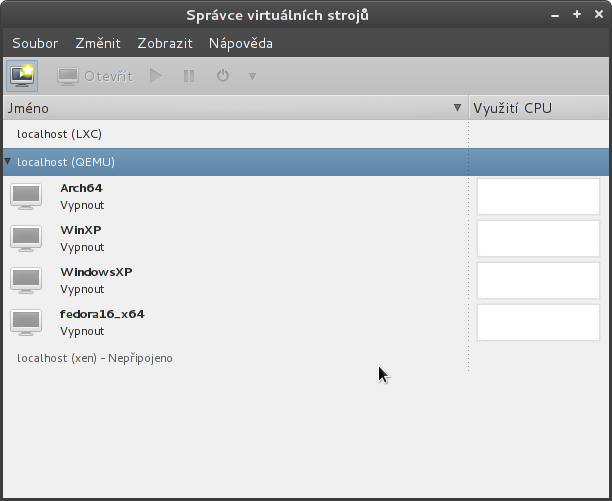
\includegraphics[width=12cm]{obr/vmm}
  \caption{Základní ono Virtual Machine Manageru.}
  \label{obr:vmm}
\end{figure}
\begin{figure}[h!]
  \centering
  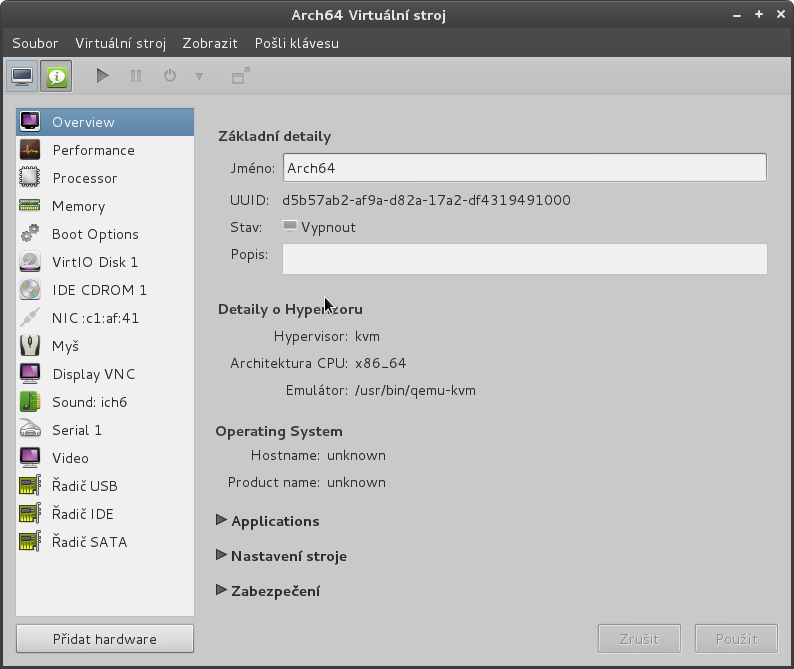
\includegraphics[width=12cm]{obr/vmmc}
  \caption{Okno pro konfiguraci virtuálního stroje.}
  \label{obr:vmmc}
\end{figure}
\newpage
Instalace Virt-manager je snadná, jelikož je součástí komunitního repositáře a není třeba jej nijak upravovat, stačí jej nainstalovat pomocí nástroje pro správu balíčků \texttt{pacman}, případně stejně dobře poslouží i již zmiňovaný \texttt{yaourt}, který je nadstavbou a umí pracovat i s normálními repozitáři.
\subsection{Konfigurace a použití}
\subsubsection{\xen}
Aby bylo možné používat, pro práci s Xen hypervizorem, Virt-manager, je zapotřebí mít nainstalován a spuštěn libvirt démon. Démon je součástí balíčku libvirt a démoni se v Arch Linuxu spouští příkazem \verb!rc.d start !\textit{\texttt{název}\texttt{\_}\texttt{démona}}. V našem případě by jsme tedy spustili příkaz \verb!rc.d start libvirtd!. Krom libvirt démona je potřeba nastartovat i další démony zajišťující běh Xen služeb. Jsou to démoni \texttt{xencommons} a \texttt{xend}. Případně \texttt{xendomains}, který má na starost automatické nastartování nainstalovaných DomU hostů.

Pozor na fakt, že v základním nastavení by nám libvirt neuměl komunikovat s Xen démonem. proto poprvé než spustíme démony, musíme xend nakonfigurovat. Celá konfigurace spočívá v nastavení (odkomentování) jednoho (dvou) řádků v souboru \verb!/etc/xen/xend-config.sxp!. Po úpravě a odstranění komentářů výsledný konfigurační soubor vypadá následovně:
\begin{alltt}
  \textbf{(xend-http-server yes)}
  \textbf{(xend-tcp-xmlrpc-server yes)}
  (xend-relocation-server yes)
  (xend-relocation-hosts-allow '^localhost$ ^localhost\textbackslash\textbackslash.localdomain$')
  (network-script network-bridge)
  (vif-script vif-bridge)
  (dom0-min-mem 196)
  (enable-dom0-ballooning yes)
  (total_available_memory 0) 
  (dom0-cpus 0)
  (vncpasswd '')
\end{alltt}

Tučně jsou zvýrazněny ty řádky, které bylo třeba odkomentovat. Po této změně a nastartování výše zmíněných démony, by již mělo jít použít Virt-manager ke správě DomU hostů.

Samotný postup vytvoření nového virtuálního stroje se pomocí Virt-manageru u jednotlivých virtualizací skoro neliší, takže si jej podrobněji ukážeme později v textu popisujícím konfiguraci KVM. Xen hosti se dají ovládat i pomocí několika dalších nástrojů. Tím úplně základním je příkaz \texttt{xm}, který je přímo součástí xenu. Jeho kompletní seznam možných operací a parametrů si vypíšeme příkazem \texttt{xm help}. Ty nejpoužívanější a nejdůležitější jsou po vypsání nápovědy uvedeny jako první. Jedná se o příkazy pro vytváření a mazání DomU hostů, jejich nastartování a vypnutí atd. Na obrázku \ref{fig:xm} vidíme několik prvních z nich.

Ačkoliv jsem po většinu času využíval kombinaci libvirt a Virt-manager, tak občas se mi stalo, že se mi ve Virt-manageru přestali zobrazovat běžící hosti. Potom bylo potřeba se na ně připojit právě pomocí utility xm. Buď pomocí příkazu \verb!xm console název_hosta! pokud byl host správně nastaven a měl spuštěný terminál, nebo případně pomocí VNC protokolu příkazem \verb!xm vncviewer název_hosta!. Aby bylo možné použít VNC spojení, je třeba mít nainstalovaný balíček \texttt{tightvnc}.
\begin{figure}[h!]
  \centering
\begin{alltt}
    console              Attach to <Domain>'s console.                     
    vncviewer            Attach to <Domain>'s VNC server.                  
    create               Create a domain based on <ConfigFile>.            
    new                  Adds a domain to Xend domain management           
    delete               Remove a domain from Xend domain management.      
    destroy              Terminate a domain immediately.                   
    domid                Convert a domain name to domain id.               
    domname              Convert a domain id to domain name.               
    dump-core            Dump core for a specific domain.                  
    list                 List information about all/some domains.          
    mem-max              Set the maximum amount reservation for a domain.  
    mem-set              Set the current memory usage for a domain.        
    migrate              Migrate a domain to another machine.              
    pause                Pause execution of a domain.                      
    reboot               Reboot a domain.                                  
    rename               Rename a domain.                                  
    reset                Reset a domain.                                   
    restore              Restore a domain from a saved state.              
    resume               Resume a Xend managed domain                      
    save                 Save a domain state to restore later.             
    shutdown             Shutdown a domain.                                
    start                Start a Xend managed domain
    \dots
\end{alltt}
\caption{Výpis několika prvních podpříkazů xm utility.}
  \label{fig:xm}
\end{figure}
\subsubsection{KVM}
U KVM je situace o něco jednoduší, jelikož zde není potřeba nic konfigurovat. Jediné co je potřeba pro správnou funkčnost libvirt a Virt-manager, jsou načtené moduly \texttt{kvm} a \texttt{kvm-amd} nebo \texttt{kvm-intel}. Potom už nám nic nebrání ke spuštění libvirt démona a následného spuštění Virt-manageru, kde si po vytvoření spojení s KVM, můžeme spravovat naše virtuální stroje. Jak to přesně provést to si teď popíšeme a ukážeme na několika obrázkách.
\begin{figure}[h!]
  \centering
  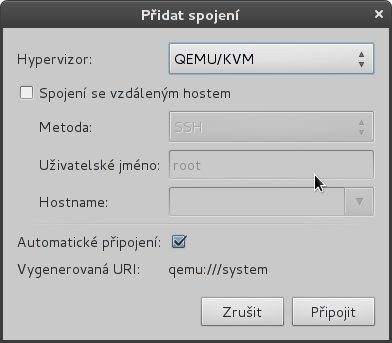
\includegraphics[width=12cm]{obr/vmmconnection}
  \caption{Okno pro nastavení spojení s hypervizorem.}
  \label{obr:vmmconnection}
\end{figure}

Po spuštění Virt-manageru se nám zobrazí hlavní okno (obrázek \ref{obr:vmm}). V tomto okně zvolíme v menu \emph{soubor} položku \emph{Přidat spojení\dots}. Tím se nám zobrazí dialogové okno jako na obrázku \ref{obr:vmmconnection}. Zde si zvolíme typ hypervizoru, který chceme používat (KVM, XEN, LXC\dots). V našem případě to bude varianta QEMU/KVM.

Dále zde můžeme nastavit zda chceme spravovat virtuální stroje bežící na tomto stroji, nebo na některém vzdáleném pomocí SSH protokolu. Jelikož v mém případě se vše testuje na jednom stroji, tak nechám možnost \emph{Spojení se vzdáleným hostem} odškrtnutou. 

Poslední co se zde dá nastavit je možnost automatického připojování v případě zapnutí Virt-manageru. Jelikož testuji několik různých virtualizačních nástrojů a ne všechny mohou běžet současně, je pro mě lepší tuto volbu nechat vypnutou a startovat si spojení na žádost (poklepáním na příslušný záznam spojení v hlavním okně). Pokud je vše správně nastaveno měly by se po spojení načíst existující virtuální stroje (pokud samozřejmě již máme nějaké vytvořené).

Samotná tvorba virtuálních strojů je velmi snadná. Slouží k tomu průvodce, který se spustí první ikonkou v nástrojové liště (ikonka počítače s šipkou a hvězdičkou). Tento průvodce nás postupně provede přidáním nového virtuálního stroje (název, určení typu OS, architektury, odkud instalovat, velikosti disků, paměti a počet použitých CPU jader\dots). Jednotlivými kroky se zde podrobně zabývat nebudu, jelikož je to mimo rozsah této práce.

Tak jako u Xenu i KVM se dá ovládat bez použití Virt-manageru. Jak už jsem psal KVM je silně svázáno s Qemu, takže se dá používat v podstatě úplně stejně. Jen s tím rozdílem že se příkazu \texttt{qemu} předá parametr (v nejnovějších verzích už není pravda, akcelerace je automaticky zapnuta), který zapíná KVM akceleraci. Krom konzolového \texttt{qemu} se dají vcelku snadno použít i různé grafické nadstavby jako je Aqemu nebo Qemu-launcher. Další možností jak KVM ovládat (spíše do budoucna) je utilita linux-kvm \footnote{\url{https://github.com/penberg/linux-kvm}}, která je momentálně ještě ve vývoji a nepodařilo se mi ji pořádně zprovoznit.
\subsubsection{UML}
UML jak jsem již psal je v podstatě jádro zkompilované do tvaru normální binární aplikace. Veškerá konfigurace probíhá stejně jako u normálního jádra pomocí parametrů. S tím rozdílem že zde se jádro nespouští přes zavaděč ale přímo jako aplikace.

K tomu abychom mohli vytvořit virtuální stroj pro UML potřebujeme mít připravený obraz disku se systémem, který chceme virtualizovat. Takový disk se dá pro různé distribuce nalézt již připravený, jelikož má využití i například pro LXC, Linux-VServer nebo klidně i pro KVM a Xen. Druhá možnost je si disk připravit ručně pomocí příkazu \texttt{dd} si naalokovat potřebnou velikost, vytvořit na něm souborový systém a nahrát potřebné systémové soubory. Natažení systému na připravený disk se dá provést buď jednoduchým zkopírováním struktury existujícího systému, nebo pomocí různých nástrojů k tomu určených.

Například pro vytvoření 5\,GB obrazu s operačním systémem Arch Linux by jsme zadali následující sekvenci příkazů:
\begin{verbatim}
  [root@KozziFX kozzi]# dd if=/dev/zero of=arch_rootfs bs=1MB count=5000
  [root@KozziFX kozzi]# mke2fs -F arch_rootfs
  [root@KozziFX kozzi]# mount -o loop arch_rootfs /mnt
  [root@KozziFX kozzi]# mkdir -p /mnt/var/lib/pacman
  [root@KozziFX kozzi]# pacman -Sy base -r /mnt
  [root@KozziFX kozzi]# cd /mnt/dev
  [root@KozziFX kozzi]# mknod --mode=660 ubd0 b 98 0
  [root@KozziFX kozzi]# chown root:disk ubd0
  [root@KozziFX kozzi]# echo "/dev/ubd0 / ext2 defaults 0 0" >> /etc/fstab
  [root@KozziFX kozzi]# umount /mnt
\end{verbatim}
První pětice příkazů vytvoří obraz na který nahraje základní systém Arch Linuxu. Zajímavější jež příkaz \texttt{mknod}, který vytváří blokové zařízení \texttt{ubd0}, které je pak přidáno jako rootfs. Důvodem proč je toto potřeba je, že UML svůj emulovaný disk mapuje právě na toto zařízení, a pokud by virtualizovaný systém neobsahoval toto zařízení, nemohl by se systém nastartovat a skončilo by to hláškou kernel panic.

Dalším krokem je připravení síťové infrastruktury pro hosta, jelikož abychom mohli nějak s virtualizovaným hostem pracovat a komunikovat, určitě budeme potřebovat, aby měl připojení alespoň do naší vnitřní sítě. UML podporuje několik způsobů (typů) připojení do sítě. Asi nejsnazší je využití nástroje \texttt{vde} (Virtual Distributed Ethernet), který se hojně využívá i u dalších podobných nástrojů jako je UML.

Jediné co je potřeba udělat aby v UML hostovi síť fungovala jsou tyto tři příkazy:
\begin{verbatim}
  [root@KozziFX kozzi]# modprobe tun
  [root@KozziFX kozzi]# vde_switch -tap tap0 -daemon -mod 660 -group users
  [root@KozziFX kozzi]# ip addr add 192.168.100.251/24 dev tap0
\end{verbatim} 

Kde první příkaz nahraje modul pro podporu tuntap zařízení, druhý příkaz vytvoří síťové zařízení \texttt{tap0}, kterému nastaví práva pro skupinu users. Třetí příkaz zařízení \texttt{tap0} přidělí IP adresu. Pokud vše jde jak má, tak potom už by jen mělo stačit hostovi nastavit IP adresu ze stejného rozsahu. A virtuálního hosta spustit s přepínačem říkajícím aby se použil typ sítě vde (parametr \texttt{eth0=vde}).

Pokud již máme připravený hostův disk a nastavenou síť můžeme jej spustit příkazem \texttt{vmlinux}. Tento příkaz se v různých distribucích může jmenovat odlišně, často se jmenuje pouze \texttt{linux}.
\begin{verbatim}
 [kozzi@KozziFX kozzi]# vmlinux mem=2048M ubda=arch_rootfs eth0=vde
\end{verbatim}
\subsubsection{VirtualBox}
VirtualBox má ze všech zmiňovaných nástrojů nejpropracovanější rozhraní pro ovládání. Obsahuje jak konzolové nástroje tak i perfektní grafickou nadstavbu. K tomu aby mohl být využít plný potenciál VirtualBoxu je potřeba načíst moduly \texttt{vboxdrv}, \texttt{vboxpci}, \texttt{vboxnetadp} a \texttt{vboxnetflt}. To je co se konfigurace týče vše.

Teď už jen stačí spustit VirtualBox a naklikat si vše potřebné. Což je v tomto nástroji opravdu velmi intuitivní a zvládne to skoro kdokoliv, kdo má alespoň základní technické znalosti. Po instalaci virtuálního počítače je velmi vhodné do něj doinstalovat VirtualBox rozšíření hosta, která velmi zpříjemňují práci s virtualizovaným strojem.
\subsubsection{LXC}
Samotné LXC nevyžaduje žádnou další konfiguraci, vše je přímo připraveno k použití. Jediné co je potřeba,tak jako u UML, je mít připravený systém, který chceme virtualizovat. Na rozdíl od UML se zde nevyužívá obraz ale přímo adresář, obsahující daný systém, který se použije jako root systému. Předpřipravený obraz se dá připojit do adresáře a ten následně použít.

Já jsem si pro svoje testování vytvořil adresář \texttt{/vservers} s podadresáři \texttt{/vservers/ArchV} a \texttt{/vservers/FedoraV}. Do těchto dvou adresářů jsem si připojil obraz Fedora Core 16, který jsem stáhl již připravený z internetu\footnote{\url{http://fs.devloop.org.uk/filesystems/Fedora16/Fedora16-AMD64-root_fs.bz2}}, a obraz Arch Linuxu. Jako obraz Arch Linuxu jsem použil již připravený obraz, který jsem si vytvořil pro UML.

Následně jsem vytvořit konfigurační soubory lxc-arch.conf \ref{lxcarch} a lxc-fedora.conf \ref{lxcfedora} obsahující základní údaje nutné k vytvoření virtuálního systému.

Samotné vytvoření kontejnerů se provádí příkazem \texttt{lxc-create} s parametry pro určení názvu kontejneru a konfiguračního souboru. V mém případě příkazy pro vytvoření kontejnerů pro virtuální systémy Arch a Fedora vypadaly následovně:
\begin{verbatim}
  lxc-create -n FedoraV -f lxc-fedora.conf
  lxc-create -n ArchV -f lxc-arch.conf
\end{verbatim}

Spuštění virtuálních systému se provádí příkazem \texttt{lxc-start -n \emph{název\_kontejneru}} a~ukončení běhu systému se provádí analogicky příkazem \texttt{lxc-stop -n \emph{název\_kontejneru}}. Pokud se daný kontejner zasekne a nejde normálně ukončit existuje zde i příkaz \texttt{lxc-kill}, který jej natvrdo ukončí. Dalšími užitečnými příkazy jsou \texttt{lxc-info} a \texttt{lxc-ls}.
\subsubsection{Linux-VServer}
Jelikož je Linux-VServer technologicky velmi podobné řešení jako LXC, použil jsem již připravené obrazy Arch Linuxu a Fedory, které nebylo třeba je nijak modifikovat.
Oproti LXC je zde o něco více práce s nastavením a tvorbou kontejnerů. Prvně je třeba spustit několik podpůrných démonů, kteří připraví systém, tak aby šlo spustit virtuální systémy. Jedná se o následující démony (\texttt{vprocunhide}, \texttt{util-vserver} a \texttt{vservers-default}). Po spuštění těchto démonů už je možné začít pracovat s Linux-VServer podobně jako s LXC. Na rozdíl od LXC je zde na všechno jen jeden příkaz nazvaný \texttt{vserver}, který jako druhý parametr očekává název kontejneru a za ním následuje druhý parametrem značící prováděnou akci nad kontejnerem. Samotné vytvoření kontejnerů se provede příkazy:
\begin{verbatim}
  vserver ArchV build -m skeleton --interface br0:192.168.100.7  --flags \
   lock,virt_mem,virt_uptime,virt_cpu,virt_load,sched_hard,hide_netif \
   --initstyle plain --context 7
  vserver FedoraV build -m skeleton --interface br0:192.168.100.9 --flags \
   lock,virt_mem,virt_uptime,virt_cpu,virt_load,sched_hard,hide_netif \
   --initstyle plain --context 9

\end{verbatim}

Linux-VServer v základu očekává své virtuální hosty v adresáři \texttt{/vservers/název\_hosta}. Jelikož jsem si tyto adresáře již připravil při konfiguraci LXC, byli použity již připravené systémy.

Samotné spuštění probíhá pomocí příkazu \verb!vserver !\texttt{\textit{název\_hosta} start}. Po nastartování virtuálního systému jej můžeme ovládat buď pomocí SSH pokud je správně nastavená síť, nebo pomocí lokální konzole virtuálního systému. Do té se přepneme příkazem \verb!vserver !\texttt{\textit{název\_hosta} enter}. Pokud již virtuální server nepotřebujeme a chceme jej zastavit, použijeme příkaz \verb!vserver !\texttt{\textit{název\_hosta} stop}.
Je tu ještě jeden příkaz \texttt{vserver-stat}, který je velmi užitečný pro zjišťování stavů virtuálních systémů.

Veškerá konfigurace kontejneru se dá nastavovat pomocí konfiguračních souborů. Ty se nacházejí v adresáři \texttt{/etc/vservers/\textit{název\_hosta}} pro jednotlivý kontejner a v adresáři \texttt{/etc/vservers/.defaults} pro všechny kontejnery. Například velmi užitečné je si přidat do kontejneru loop rozhraní. To provedeme vytvořením adresáře \texttt{\textit{číslo}} v adresáři \texttt{/etc/vservers/\textit{název\_hosta}/interfaces/}. Kde \texttt{\textit{číslo}} je číslo označující rozhraní. Pokud tedy již máme přidáno jedno rozhraní, tak zde bude existovat adresář s názvem \texttt{0} a vytvořením adresáře \texttt{1} vytvoříme další rozhraní. Vytvoření adresáře nestačí, a je potřeba v něm vytvořit minimálně soubory \texttt{dev}, \texttt{ip} a  \texttt{prefix}. Tyto soubory budou obsahovat jak názvy napovídají název rozhraní, IP adresu a prefix sítě. V mém případě jsem zadal tyto příkazy:
\begin{alltt}
  mkdir /etc/vservers/\emph{název\_hosta}/interfaces/1
  echo "lo" > /etc/vservers/\emph{název\_hosta}/interfaces/1/dev
  echo "127.0.0.1" > /etc/vservers/\emph{název\_hosta}/interfaces/1/ip
  echo "32" > /etc/vservers/\emph{název\_hosta}/interfaces/1/prefix
\end{alltt}

Pokud bychom chtěli nastavit automatické nastartování virtuálních systému při startu hostitele, musíme přidat výše zmíněné démony do sekce \texttt{DAEMONS} v souboru \texttt{/etc/rc.conf}. To nám zajístí jejich spouštění při startu hostitele. A potom je ještě třeba jednotlivé virtuální systémy označit, aby se také sami spustili. To se provede příkazem:
\begin{alltt}
  echo default > /etc/vservers/\emph{název\_hosta}/init/mark
\end{alltt}


\chapter{Výkonnostní testy}
\section{Metodika měření, aneb co a jak se bude měřit}
V této předposlední kapitole si řekneme něco málo o tom, jak probíhalo samostatné testování. Představím nástroje, jenž byli použity a nakonec si ve formě grafů ukážeme, jak obstáli naši kandidáti v jednotlivých testech.
\subsection{Virtualizované systémy a jejich konfigurace}
Jak už jsem psal v předešlé kapitole jako operační systém pro hostitele jsem si zvolil Arch Linux. V případě hosta jsem se rozhodl hned pro dvě distribuce. Důvodem bylo zjistit, zda rozdílné distribuce běží ve virtualizovaném prostředí odlišně. Jedním vybraným kandidátem je opět Arch Linux a jako další byla zvolena Fedora Core 16. O výhodách těchto systémů jsem se již zmiňoval, takže se zde o nich znovu nebudu rozepisovat.

Obě tyto distribuce byli ponechány během testování v základním nastavení. Tím mám namysli, že zde nebyli prováděny žádné zásahy, které by ovlivňovali jejich výkonnost v testech (změna konfigurace jádra a podobně). Samozřejmě po dobu testování nebyly na těchto systémech prováděny aktualizace, tak aby všechny výsledky byly co nejvěrohodnější. Jediné úpravy byly ty, které přímo souviseli s podporou dané virtualizační technologie, jako například doinstalování rozšíření pro VirtualBox atd.

U obou dvou distribucí i u všech virtualizačních technologií jsem se snažil vytvořit pokud možno co nejhomogennější prostředí. Všem virtuálním systémům bylo vždy přiděleno jen jedno jádro a 2048\,MB operační paměti.

\section{Phoronix Test Suite}
Aby bylo testování co nejpohodlnější, a aby bylo zaručeno co nejpřesnější měření, které se bude dát zopakovat. Rozhodl jsem se pro vlastní testování využít testovací software Phoronix Test Suite (dále jen PTS). PTS je nástroj a sada testů vytvořených webovým portálem Phoronix pro automatické testování na platformě Linux. Později byl nástroj rozšířen i o řadu dalších operačních systémů. Celý nástroj je napsán za pomocí skriptovacího jazyka PHP a pokud je v systému nainstalována knihovna PHP-GTK, lze použít i grafické prostředí tohoto nástroje.

\subsection{Dostupné testy}
Jednotlivé testy a testovací sady, nejsou přímo součástí PTS, ale stahují se přímo z webu, což umožňuje snadné přidávání nových testů. V době psaní této práce je dostupných něco přes 100 testů. Všechny testy jsou rozděleny do kategorií podle toho co testují (disky, procesor, systém, grafiku a další).

Každý test se skládá z několika XML souborů a pár dalších bash skriptů, což umožňuje jejich snadné přizpůsobení v případě potřeby. Díky jednoduché syntaxi a dobrému návrhu je velmi snadné si přidávat i vlastní testy.

\subsection{Způsob měření}
Každý test obsahuje počet opakování měření, které je třeba při testování provést. Následně z těchto pokusů udělá aritmetický průměr. Z těchto pokusů se počítají i další údaje, jako je standardní odchylka a chyba. V případě že je odchylka větší než 3,\%, počet pokusů se zdvojnásobí, čímž je dosažené zpřesnění výsledků. Tento postup se však provede pouze jednou. V případě zdvojnásobeného počtu pokusů se i přes větší odchylku již dále neměří a jako výsledek je určen aritmetický průměr všech naměřených hodnot.

\subsection{Zaznamenávání výsledků}
Během spouštění testu je člověk dotázán zda-li chce naměřené výsledky uložit. Pokud zvolí ne, tak jsou výsledné údaje vypsány na konzoli. V případě zvolení kladné odpovědi se testovací nástroj dále zeptá na název pod kterým má být test uložen. Také se zeptá na unikátní identifikátor, který se používá pro odlišení jednotlivých výsledků v případě uložení testu pod stejným názvem. Pokud se nevyplní je automaticky vložen aktuální datum a čas. Nakonec se ještě zeptá na podrobnější popis daného testu.

Po skončení testu opět vypíše naměřená data na obrazovku, ale krom toho je také uloží na disk ve formě XML souboru. Z tohoto XML souboru ještě navíc vygeneruje graf ve formátu SVG. Veškeré uložené výsledky všech testů se nacházejí v domovském adresáři uživatele, jenž spouštěl test, ve složce \texttt{.phoronix-test-suite/test-results/\textit{název\_testu}}.

\subsection{Popis používání}
Ovládání PTS je velmi snadné a pokud program spustíme vyběhne na nás i nápověda se seznamem možných parametrů. Během celého testování jsem potřeboval asi jen čtyři příkazy. Prvním z nich je příkaz na vypsání všech dostupných testů.
\begin{verbatim}
 phoronix-test-suite list-available-tests
\end{verbatim}
Když už známe dostupné testy je potřeba si je stáhnout a nainstalovat. To se provede příkazem \texttt{phoronix-test-suite install \textit{název\_testu}}. PTS je dokonce tak propracovaný, že během instalace zvoleného testu otestuje systém zda obsahuje veškerý potřebný software. V případě zjištění chybějící závislosti ji dokáže u několika distribucí sám doinstalovat. Pokud není schopný ji sám doinstalovat, tak oznámí na konzoli název chybějícího software.

Pokud již máte test nainstalovaný, ale chcete jej přeinstalovat můžete použít místo parametru \texttt{install} slovo \texttt{force-install}. Posledním příkazem je samotné spuštění testu:
\begin{alltt}
 phoronix-test-suite run \emph{název\_testu}
\end{alltt}

\subsection{Zvolené testy}
Jelikož PTS obsahuje spousty testů pro různé účely a z důvodů rozsahu jsem si nemohl dovolit udělat je všechny, musel jsem se rozhodnout kolik a které z nich si vybrat. Nakonec jsem se rozhodl pro 11 testů, u kterých jsem se snažil vybírat tak, aby testovali pokud možno různé aspekty výkonu virtualizovaného systému. V tabulce \ref{tab:bench} je vidět jejich přehled i s popisem co testují.
\begin{table}[ht]
\begin{center}
    \begin{tabular}{|l|l|}
      \hline
       \textbf{aio-stress} & náhodný zápis na disk \\
      \hline
       \textbf{apache} & počet zpracovaných požadavků za sekundu \\
      \hline
       \textbf{build-php} & dobu sestaveni PHP 5 \\
      \hline
       \textbf{gnupg} & dobu zašifrování 2\,GB velkého souboru \\
      \hline
       \textbf{phpbench} & sada malých testů na měření výkonu PHP \\
      \hline
       \textbf{pybench} & doba nutná k provedení sady testů napsaných v pythonu \\
      \hline
       \textbf{ramspeed} & měření rychlosti operační paměti\\
      \hline
       \textbf{stream} & komplexnější měření výkonu operační paměti \\
      \hline
       \textbf{unpack-linux} & doba nutná k rozbalení zdrojových kódů jádra Linuxu \\
      \hline
       \textbf{vpxenc} & počet snímků za sekundu při kódování do VP8 video formátu \\
      \hline
       \textbf{x264} & počet snímků za sekundu při kódování do H.264 video formátu \\
      \hline
    \end{tabular}
 \caption{Seznam použitých testů při testování hostů}
 \label{tab:bench}
\end{center}
\end{table}

\section{Vyhodnocení měření}
Na následujících grafech a tabulkách (obrázky \ref{obr:bench:aio}--\ref{obr:bench:x264}) jsou zaznamenány výsledky jednotlivých testů. Testoval jsem vždy na všech virtuálních strojích (systémech) a pro srovnání i přímo na hostiteli. Jediný rozdíl je u technologie UML, zde jsem testoval pouze Arch Linux hosta, jelikož se zprovozněním Fedory pod UML jsem měl potíže, které se mi nepodařilo uspokojivě vyřešit. A ještě jedna drobnost ohledně UML a tou je nemožnost rozchodit test kódování videa pomocí \texttt{x264} utility.

V následujících podsekcích postupně proberu naměřená data a poukáži na ty nejdůležitější věci, které se dají z grafů vyčíst. Dále zde budu používat pojmy plnohodnotná virtualizace a kontejnerová řešení. Pod pojmem plnohodnotná virtualizační řešení mám namysli technologie KVM, Xen a VirtualBox. Pod pojmem kontejnerová virtualizace si představte technologie LXC a Linux-VServer. Co se UML týče, tak to nechám samostatně a nezařazuji jej ani do jedné ze skupin (patřilo by spíše někam mezi emulátory).

\subsection{AIO-Stress}
Pokud se podíváme na výsledky tohoto test (obr. \ref{obr:bench:aio}), zjistíme že UML získal neuvěřitelně vysoké skóre. Test jsem několikrát opakoval a vždy se stejným výsledkem. Pravděpodobně se jedná o určitou chybu související se způsobem, jak má UML emulovaný svůj IO subsystém.

Další věcí které si všimneme je propad všech virtualizačních technologií vyjma UML a kontejnerové virtualizace. A to v případě Fedory i Arch Linuxu. Důvodem je, že tento test je zaměřený na asynchronií zápis, který generuje hodně I/O požadavků. A jelikož moje sestava nepodporuje virtualizaci IOMMU (někdy označováno jako PCI passthrough), musí se veškeré tyto požadavky emulovat a zpracovávat přes procesor což vede k rapidnímu snížení výkonu.

Zbytek výsledků vcelku odpovídá předpokladům, jen je dobré si všimnout že co se distribucí týče, tak má Fedora mírně navrch. to může být způsobeno rozdílnou verzí ovladače v jádře či jeho konfigurací, nebo verzí knihovny \texttt{libaio}.

\subsection{Apache}
V tomto testu (obr. \ref{obr:bench:apache}) zcela propadl UML, který zvládl obsloužit 3x až 4x méně požadavků. Důvodem bude fakt, že UML nevyužívá žádné HW akcelerace a vše běží uvnitř jednoho procesu. To způsobuje nízký výkon v určitých situacích, jako například vytváření spousty krátkých procesů a přepínání kontextu, což se v tomto testu dělo.

Z pohledu distribucí je vidět, že v případě kontejnerové virtualizace měla mírně navrch Fedora. Na druhou stranu co se plnohodnotné virtualizace týče, zde si zase lépe vedl Arch Linux, hlavně host bežící na 
KVM.

\subsection{Build PHP}
Výsledky kompilace PHP se nachází na obrázku \ref{obr:bench:buildphp}. Na první pohled jde vidět, že zde opět zcela výkonnostně propadl UML. A částečné propadl i Xen hypervizor. Ostatní řešení byly celkem vyrovnaná. Ještě si můžeme všimnout rozdílu mezi Archem a Fedoru, kde Fedora má výkonnostně mírně navrch.

\subsection{GnuPG}
Na obrázku \ref{obr:bench:gnupg} vidíme graf výkonu jednotlivých hostů při práci se šifrovacím programem GnuPG. Z grafu je patrné, že všechna řešení dosahovala velmi podobných výsledků. Drobný pokles výkonu je patrný akorát u UML a VirtualBoxu.


\subsection{PHPBench}
U PHPBench (obr. \ref{obr:bench:phpbench}) je opět nejslabší host běžící na UML. Trochu zarážející je i výkon přímo hostitele, který má druhý nejhorší výsledek. Pravděpodobně to souvisí nějak s omezením na jedno jádro, což bylo provedeno pomocí cpuset. Stejná metoda je využívána i u LXC a Linux-VServer, kde výkon není příliš odlišný od hostitele.

Dobře patrné je tu i lepší výkon hostů na nichž běží Fedora. Což není poprvé a dalo by se z toho usuzovat, že je Fedora očividně lépe odladěná. Teda až na VirtualBox kde je výkon Fedory většinou docela slabý. 

\subsection{PyBench}
Dalším testem je PyBench, který testuje sadu skriptů v Pythonu a měří jak dlouho trvá jejich běh (výsledky jsou znázorněny na obrázku \ref{obr:bench:pybench}). Tak jako u GnuPG i zde se dá říci, že jsou všichni hosti velmi vyrovnaní. Mírně zaostává jen Fedora host běžící ve VirtualBoxu a celkově je zde nepatrně lepší výkon hostů na nichž běží Arch Linux (pravděpodobně je zde rychlejší verze Pythonu).
\subsection{RAMspeed}
Zde už je na graf (obr. \ref{obr:bench:ramspeed}) mírně pestřejší, ale i přesto zde není vidět žádný vyložený propad. Nejhůře v tomto testu dopadl Xen host na němž běžel Arch Linux, následovaný Fedorou bežící ve VirtualBoxu. Nejvýkonější se ukázali řešení využívající kontejnery. V tomto testu pak zejména řešení Linux-VServer s Fedora hostem.
\subsection{Stream}

Stream je další z testů zaměřených na testování paměti RAM. Na rozdíl od testu RAMspeed toho testuje víc. Při pohledu na výsledky (obr. \ref{obr:bench:stream}) je opět vidět vyrovnanost všech soupeřů. Jediný kdo v každém ze čtyř testů mírně ztrácí na výkonu je kombinace VirtualBox a Fedora. Ve třech testech se na první pozici umístilo kontejnerové řešení LXC a dvakrát z toho v kombinaci s operačním systémem Fedora. Zbývající jeden test dosáhlo nejvyššího skóre paradoxně řešení s VirtualBoxem v kombinaci se systémem Arch Linux. 
\subsection{Unpack linux}
Při testování rychlosti rozbalování archívu se zdrojovými kódy jádra Linuxu na posledním místě umístil UML. Z grafu (obr. \ref{obr:bench:unpacklinux}) dále vyplývá, že s rozbalováním měly potíže i oba systémy bežící na VirtualBoxu a nejlepšího času nedosáhly ani řešení využívající Xen hypervizor. Ostatní soupeři se nelišili v rychlosti o více než sekundu.
\subsection{VP8 vpxenc}
Výkony jednotlivých systémů prezentované na obrázku \ref{obr:bench:vpxenc} bych rozdělil na dvě skupiny. Na skupinu jenž dokázala průměrně za sekundu kódovat minimálně 7,5 snímků a na ty zbylé jenž se drželi okolo 6 snímků za sekundu. Do první vítězné skupiny se řadí KVM a XEN s oběma systémy a UML. Zbytek (VirtualBox oba systémy, LXC oba systémy a Linux-VServer oba systémy) spadají do skupiny s horším hodnocením. Zcela Nejhoršího výkonu dosáhlo řešení Arch Linux plus LXC a na druhé straně nejlepšího výkonu dosáhl Arch Linux běžící jako KVM host.
\subsection{X264 encoder}
Poslední test je vyobrazen na obrázku \ref{obr:bench:x264} a ukazuje výkon jednotlivých hostů při kódování videa do formátu H.264 pomocí programu \texttt{x264}. Až na obě řešení využívající VirtualBox jako hypervizor dosáhli všichni rychlosti okolo 25 snímků za vteřinu, což je velmi slušný výkon.

\begin{figure}[ht!]
  \centering
  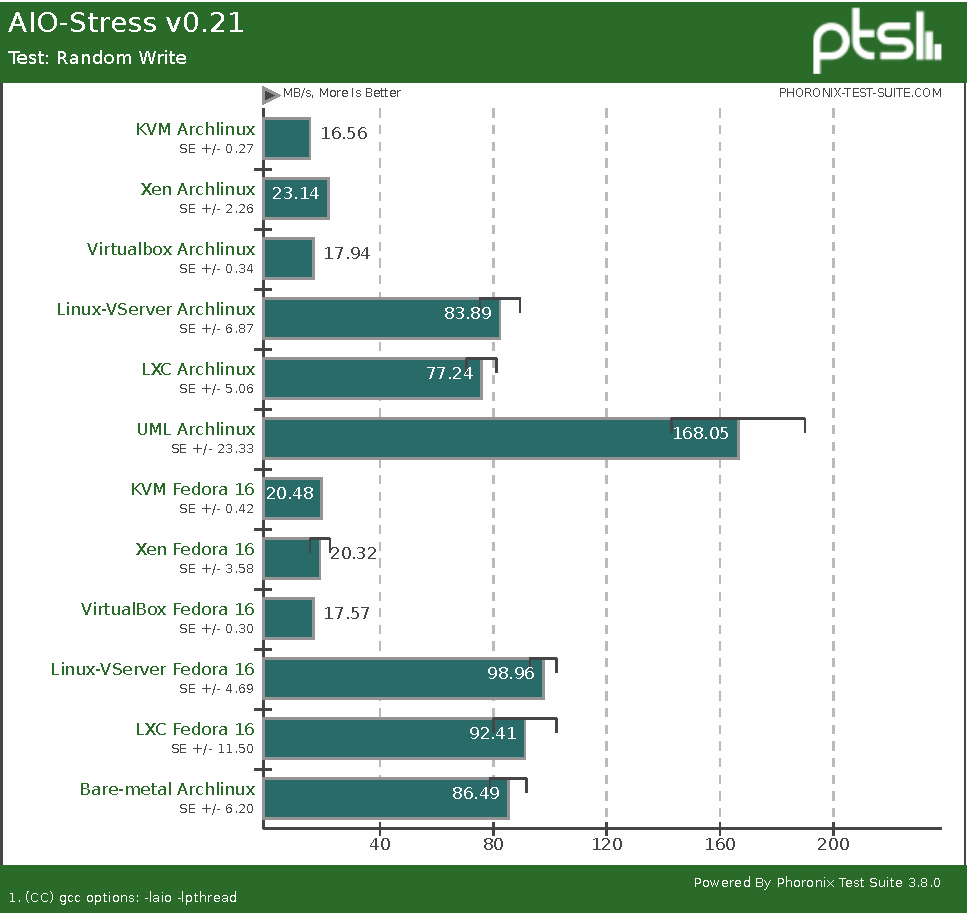
\includegraphics[width=15cm]{obr/bench/aio-stress-graph}
  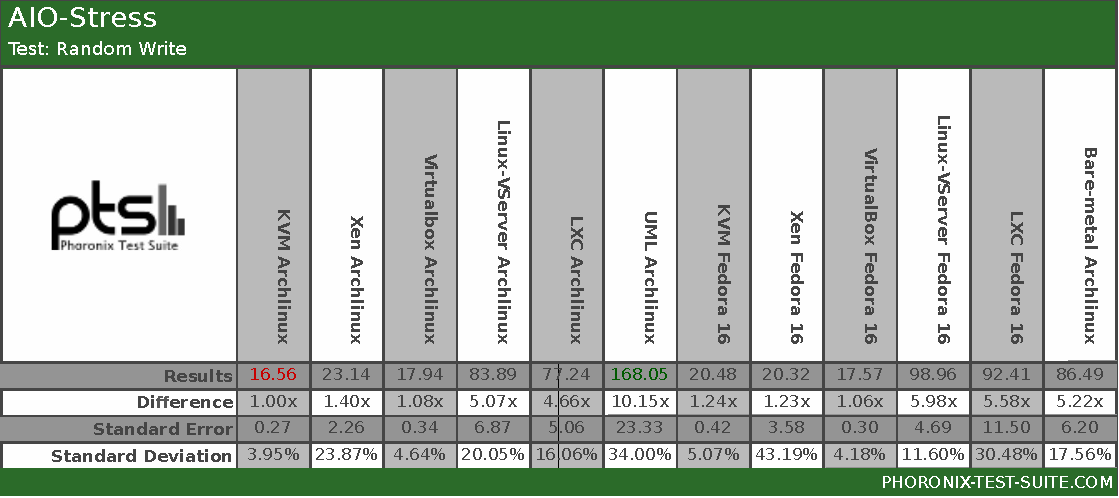
\includegraphics[width=15cm]{obr/bench/aio-stress-table}
  \caption{Výsledky AIO-Stress.}
  \label{obr:bench:aio}
\end{figure}




\begin{figure}[h!]
  \centering
  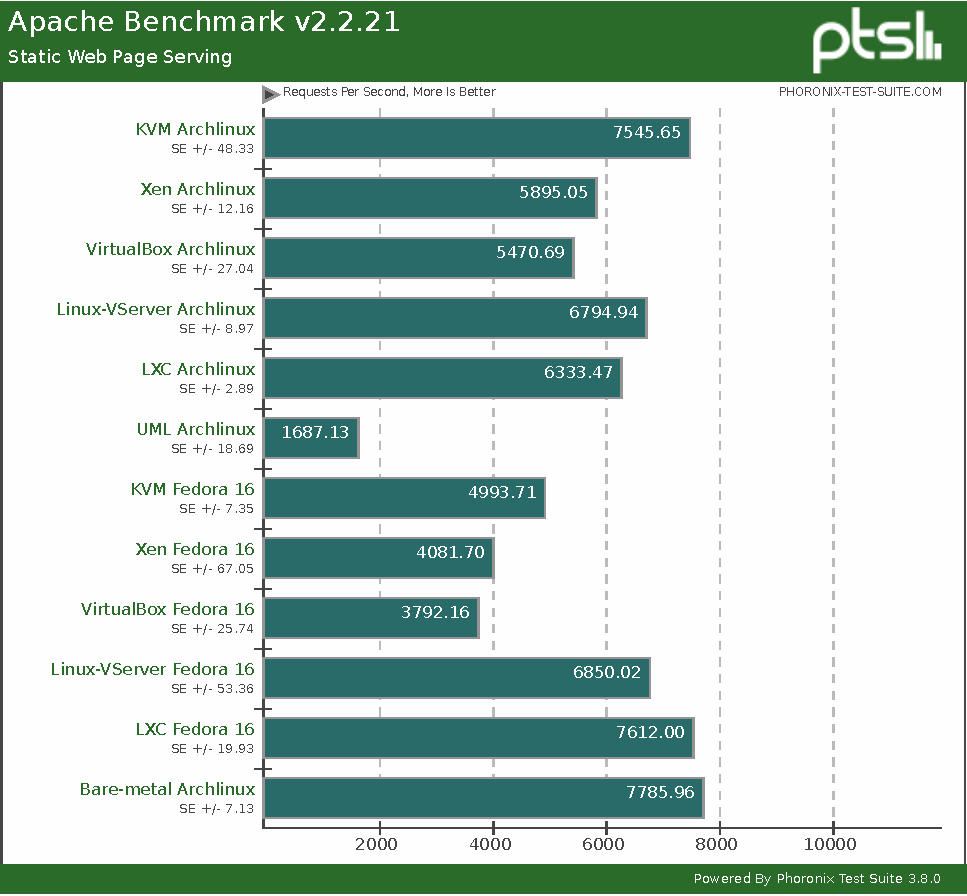
\includegraphics[width=15cm]{obr/bench/apache-graph}
  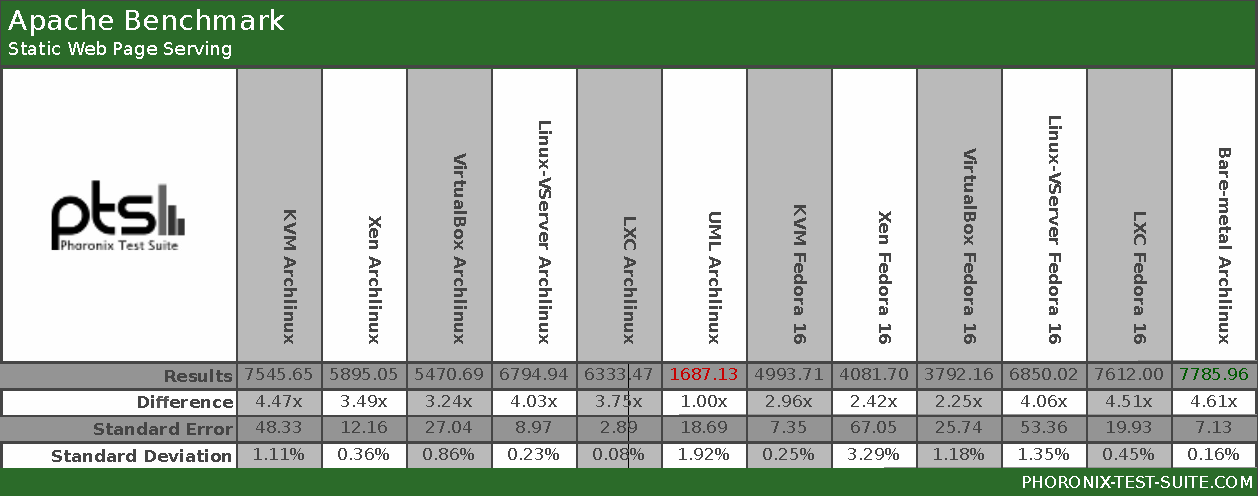
\includegraphics[width=15cm]{obr/bench/apache-table}
  \caption{Naměřené hodnoty Apache benchmarku.}
  \label{obr:bench:apache}
\end{figure}



\begin{figure}[h!]
  \centering
  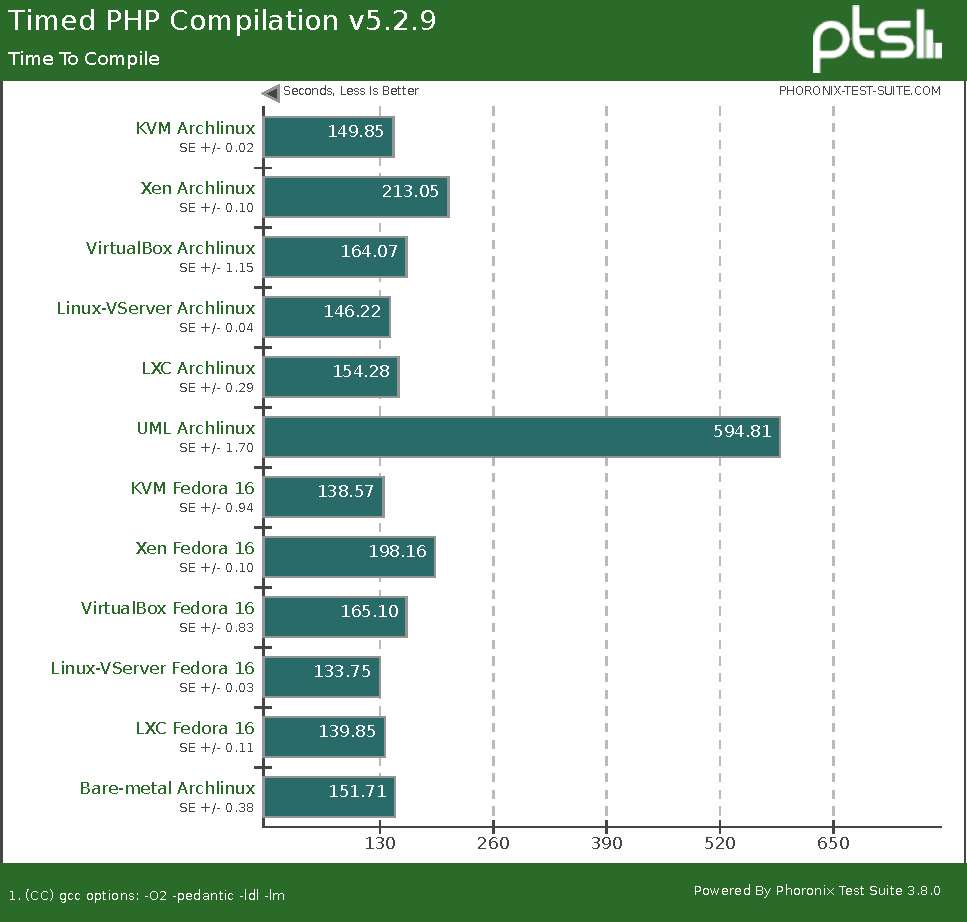
\includegraphics[width=15cm]{obr/bench/build-php-graph}
  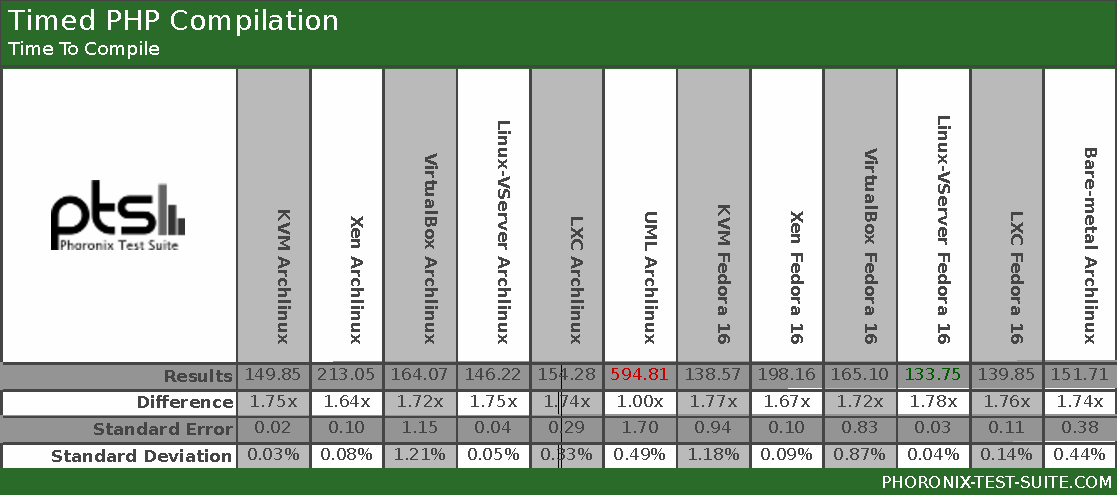
\includegraphics[width=15cm]{obr/bench/build-php-table}
  \caption{Výsledné hodnoty sestavování PHP aplikace.}
  \label{obr:bench:buildphp}
\end{figure}



\begin{figure}[h!]
  \centering
  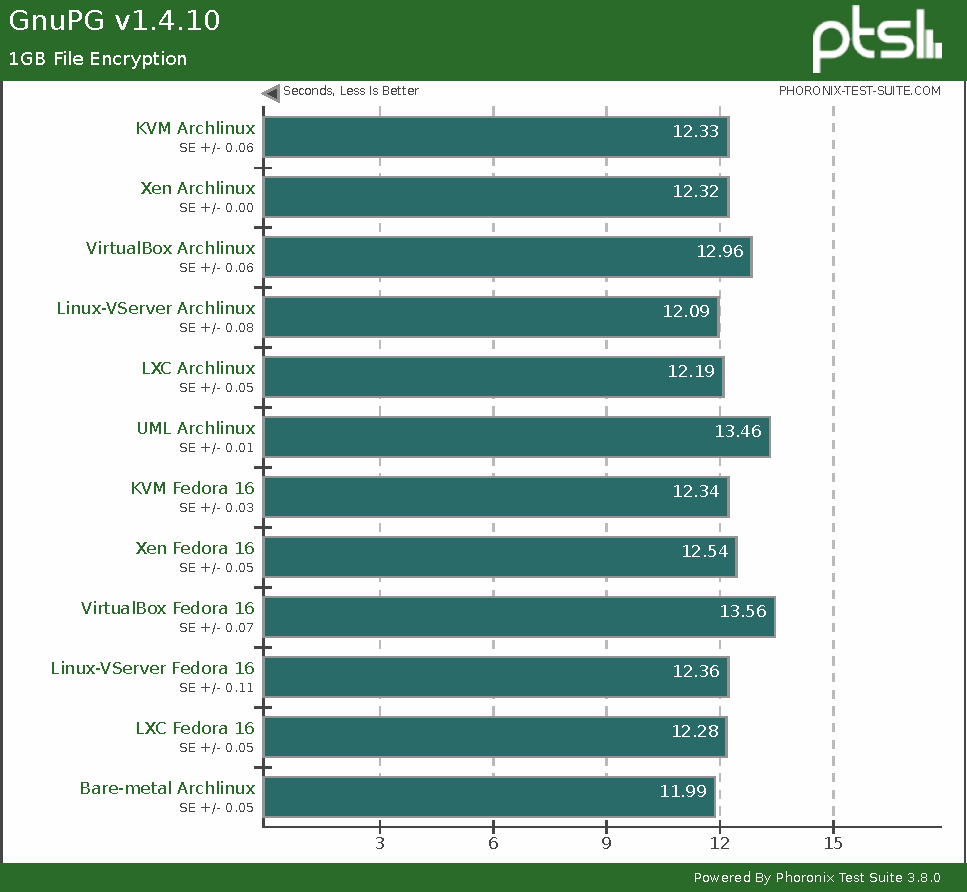
\includegraphics[width=15cm]{obr/bench/gnupg-graph}
  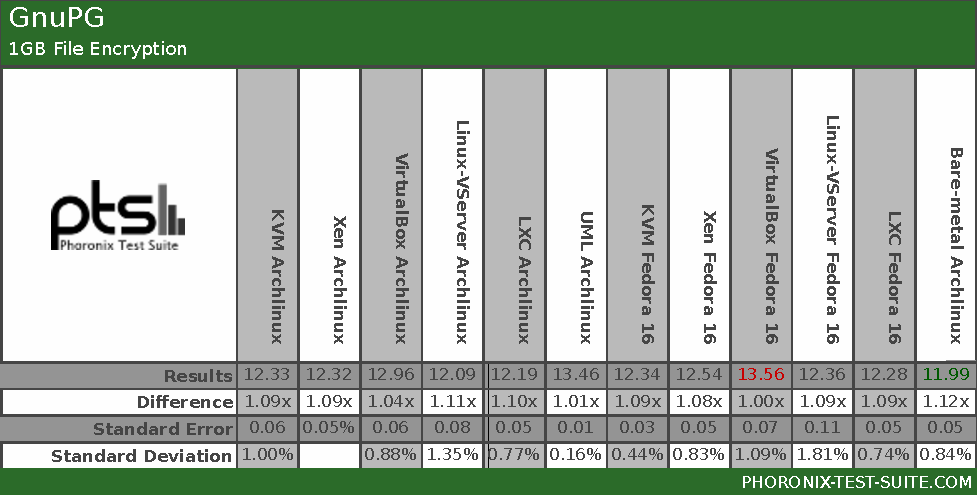
\includegraphics[width=15cm]{obr/bench/gnupg-table}
  \caption{Doba potřebná k zašifrování soubrou pomocí GnuPG.}
  \label{obr:bench:gnupg}
\end{figure}



\begin{figure}[h!]
  \centering
  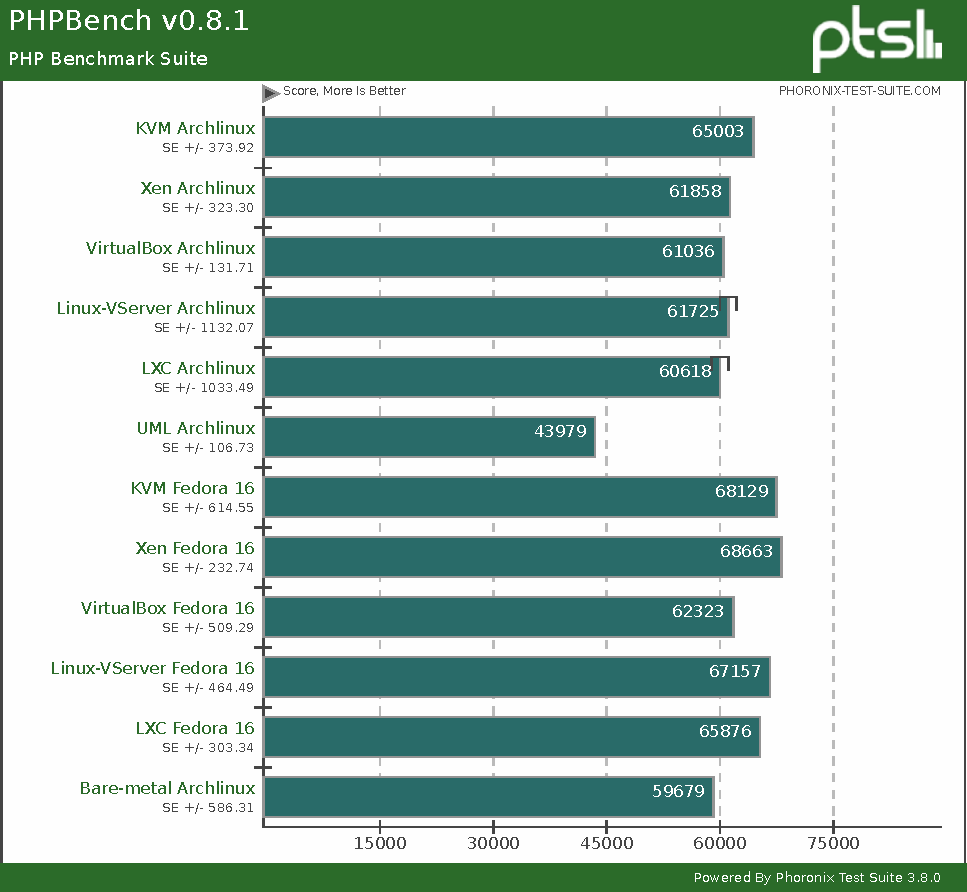
\includegraphics[width=15cm]{obr/bench/phpbench-graph}
  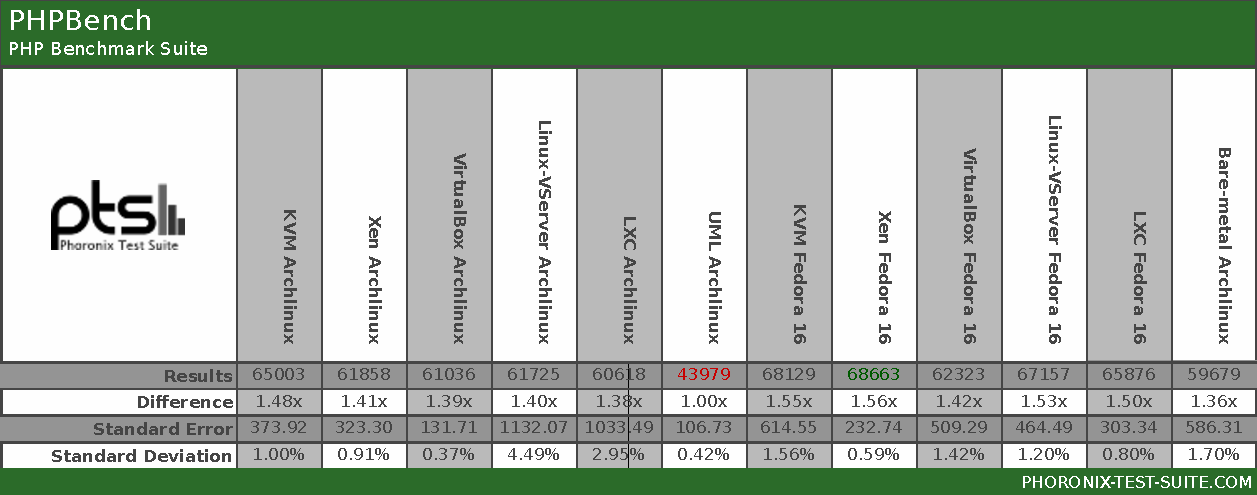
\includegraphics[width=15cm]{obr/bench/phpbench-table}
  \caption{Počet bodů získaný v PHPBench.}
  \label{obr:bench:phpbench}
\end{figure}



\begin{figure}[h!]
  \centering
  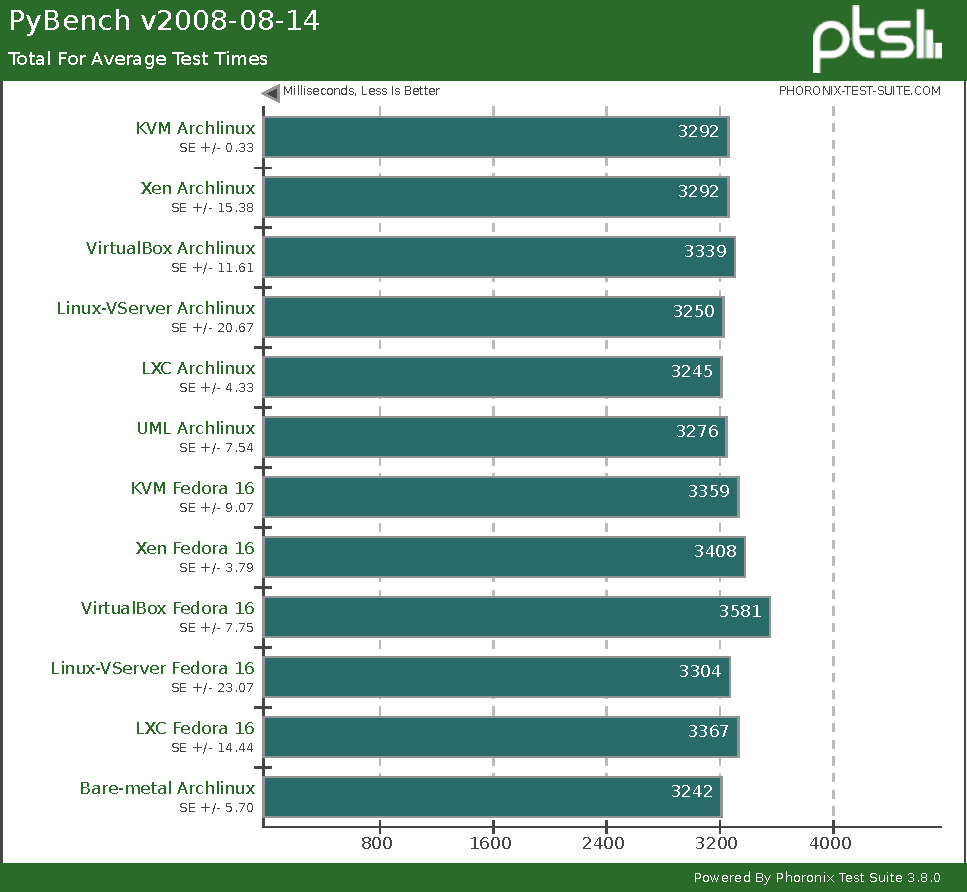
\includegraphics[width=15cm]{obr/bench/pybench-graph}
  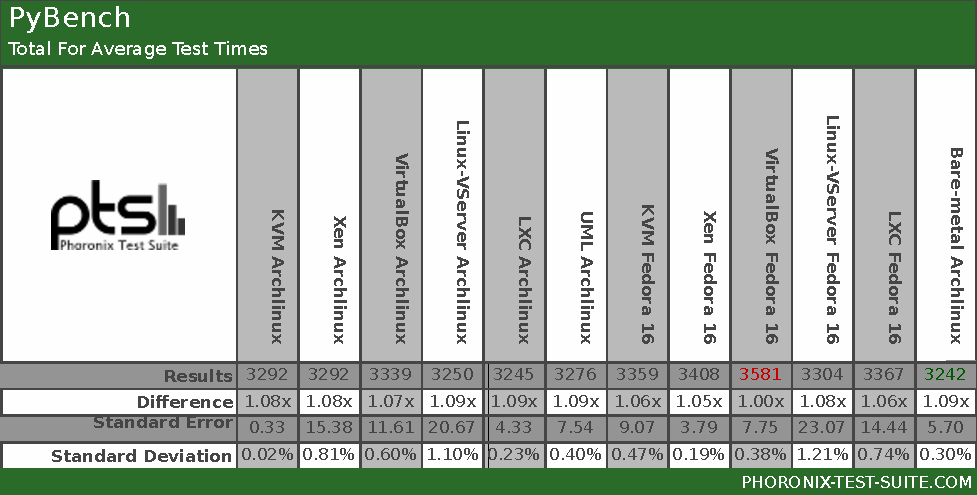
\includegraphics[width=15cm]{obr/bench/pybench-table}
  \caption{Doba nutná pro dokončení PyBench.}
  \label{obr:bench:pybench}
\end{figure}

\begin{figure}[h!]
  \centering
  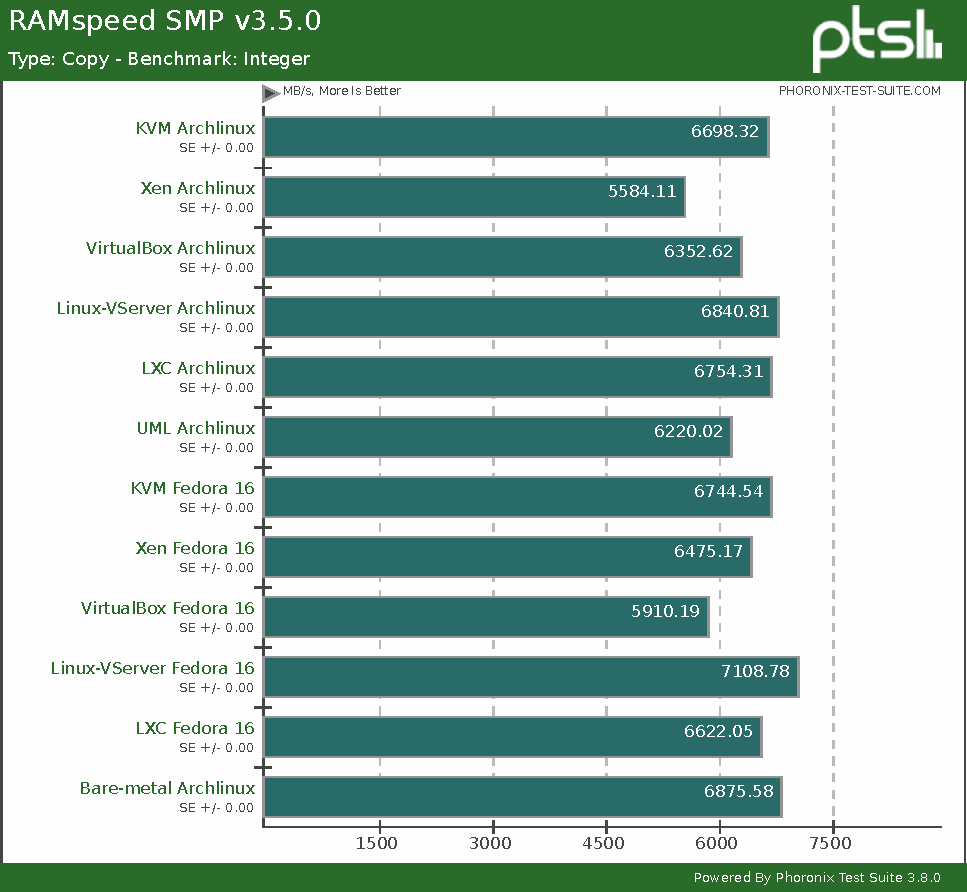
\includegraphics[width=15cm]{obr/bench/ramspeed-graph}
  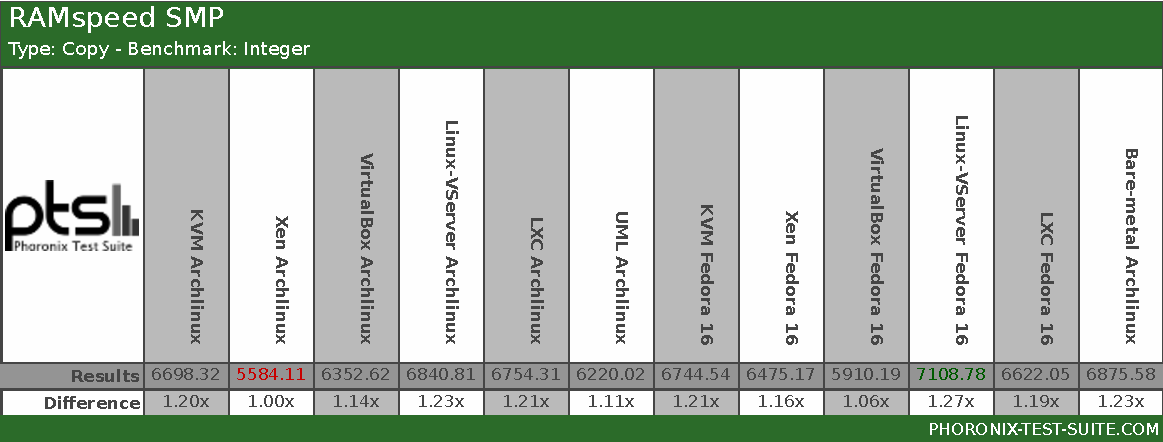
\includegraphics[width=15cm]{obr/bench/ramspeed-table}
  \caption{Rychlost kopírování celého čísla v MB/s.}
  \label{obr:bench:ramspeed}
\end{figure}



\begin{figure}[h!]
  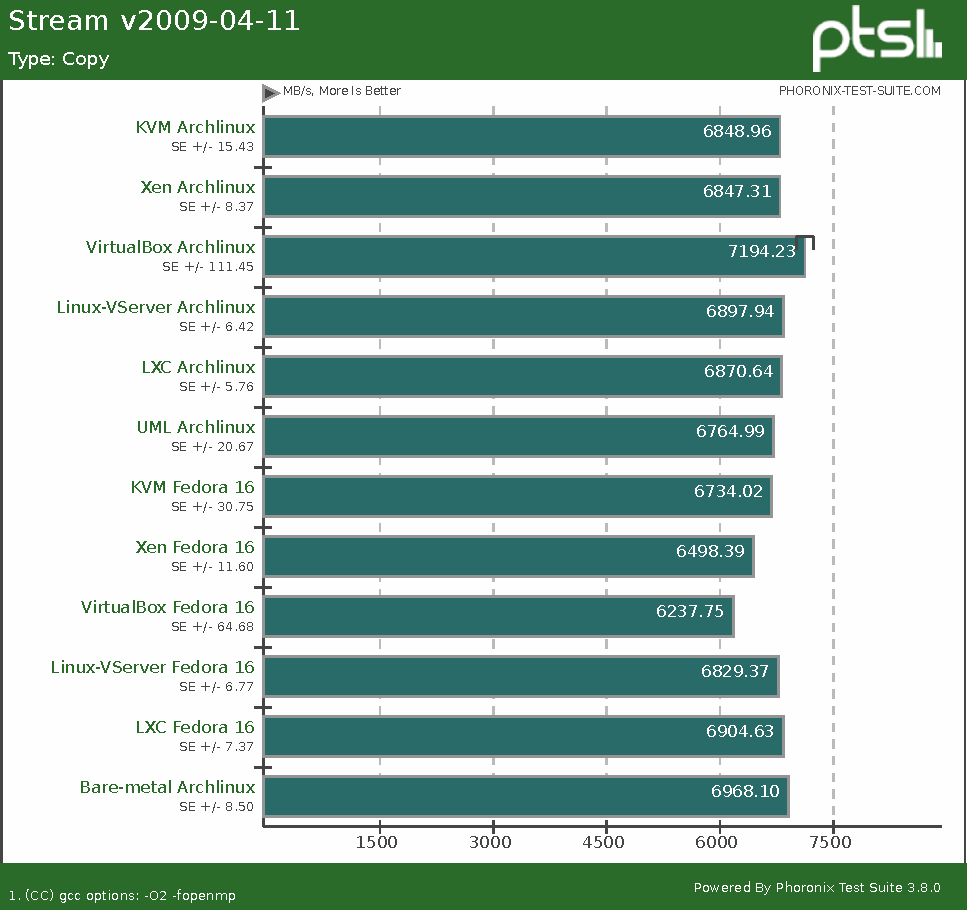
\includegraphics[width=75mm]{obr/bench/stream-graph-1}
  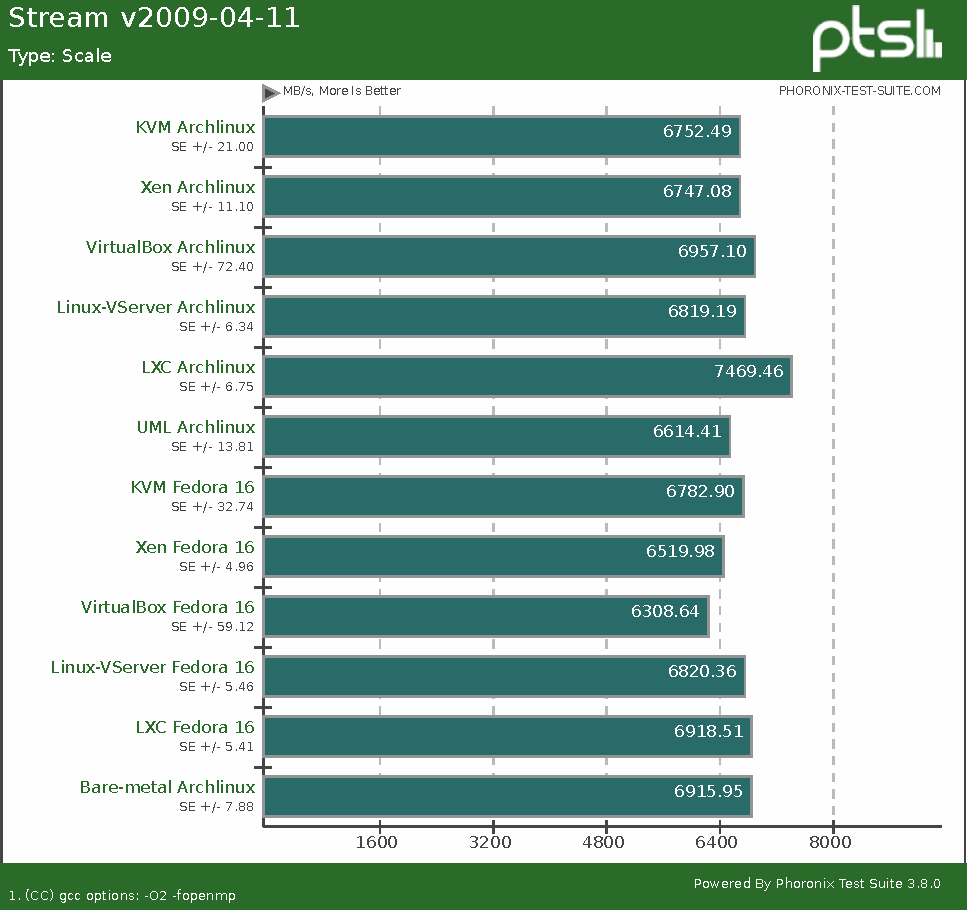
\includegraphics[width=75mm]{obr/bench/stream-graph-2}
  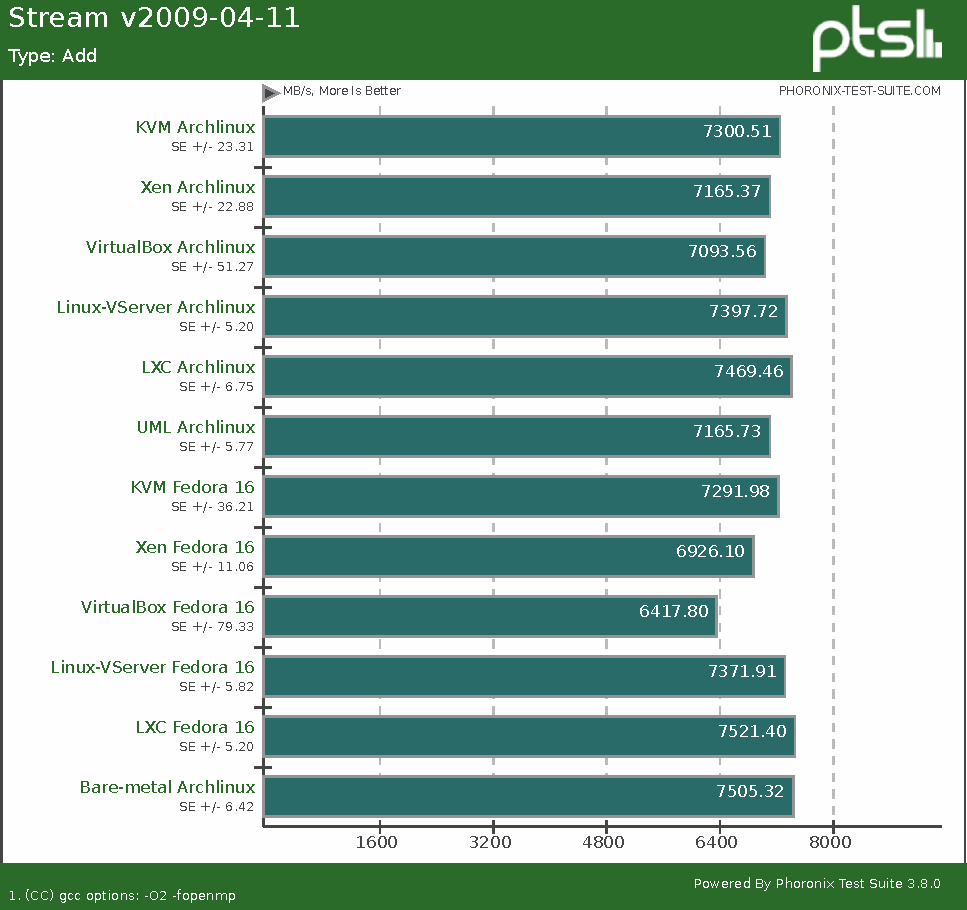
\includegraphics[width=75mm]{obr/bench/stream-graph-3}
  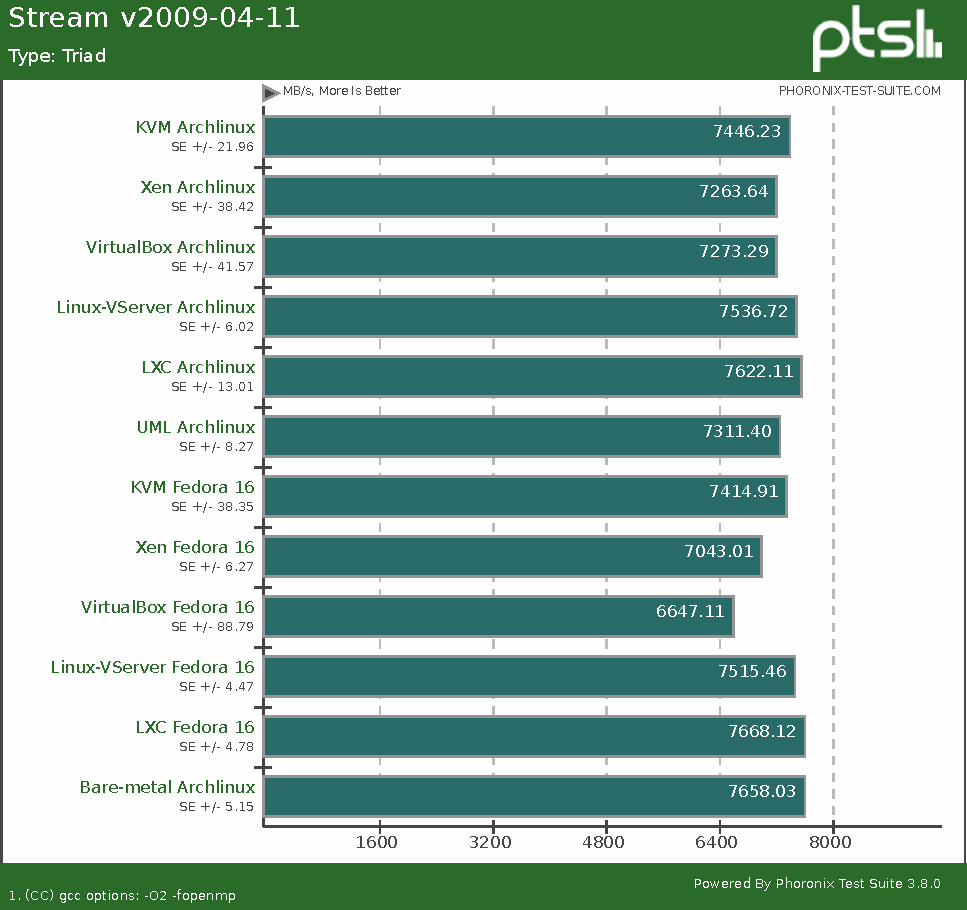
\includegraphics[width=75mm]{obr/bench/stream-graph-4}
  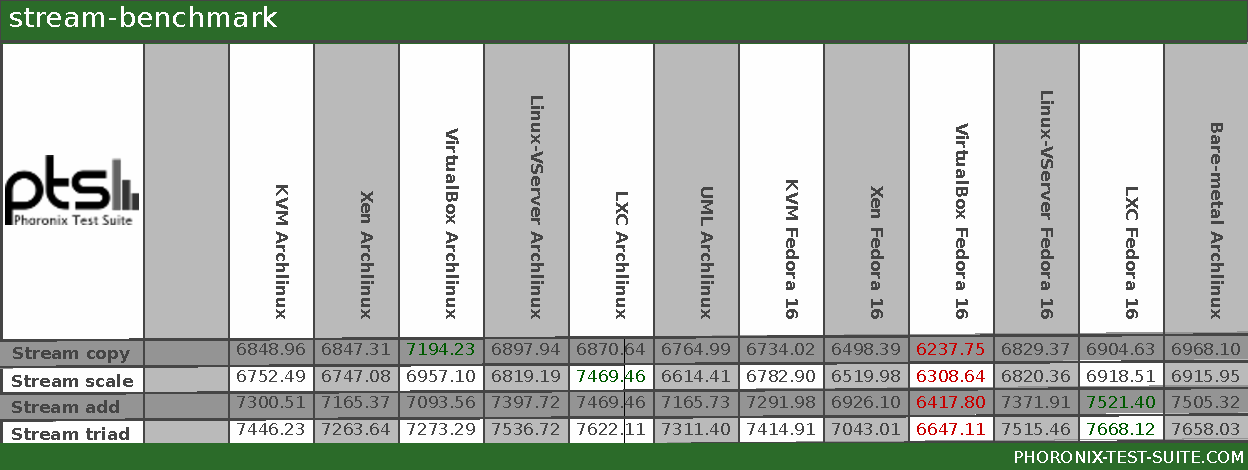
\includegraphics[width=152mm]{obr/bench/stream-table}
  \caption{Rychlost operací s operační pamětí.}
  \label{obr:bench:stream}
\end{figure}


\begin{figure}[h!]
  \centering
  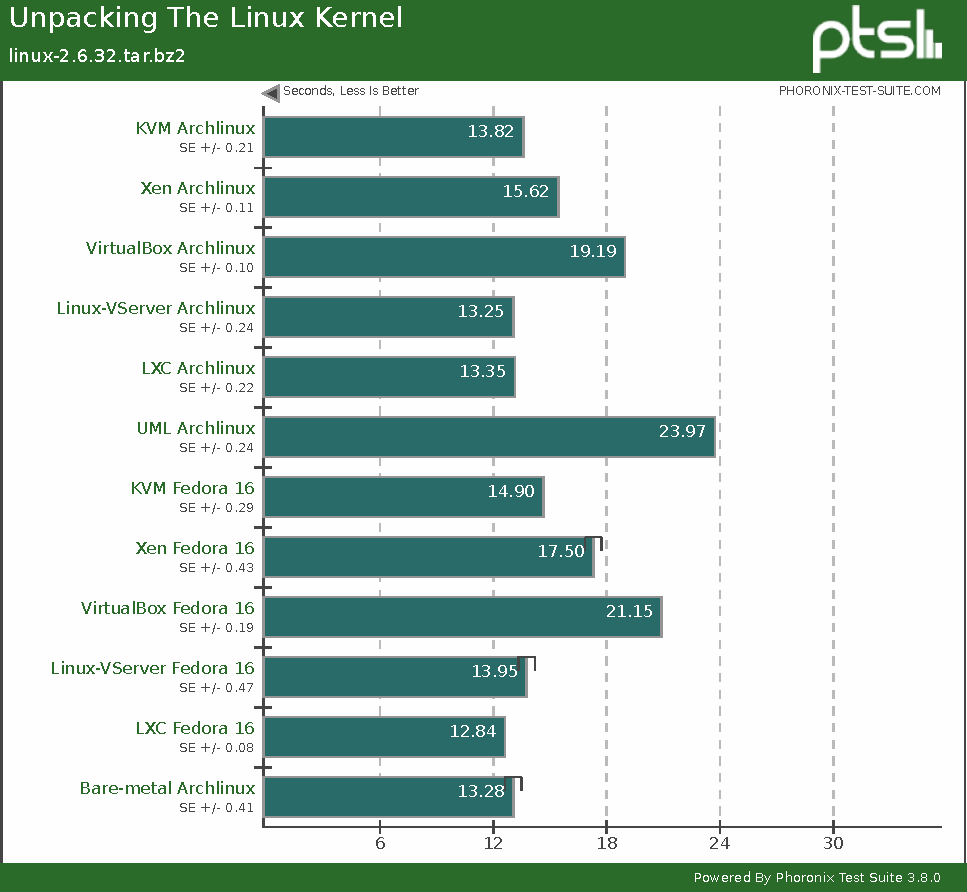
\includegraphics[width=15cm]{obr/bench/unpack-linux-graph}
  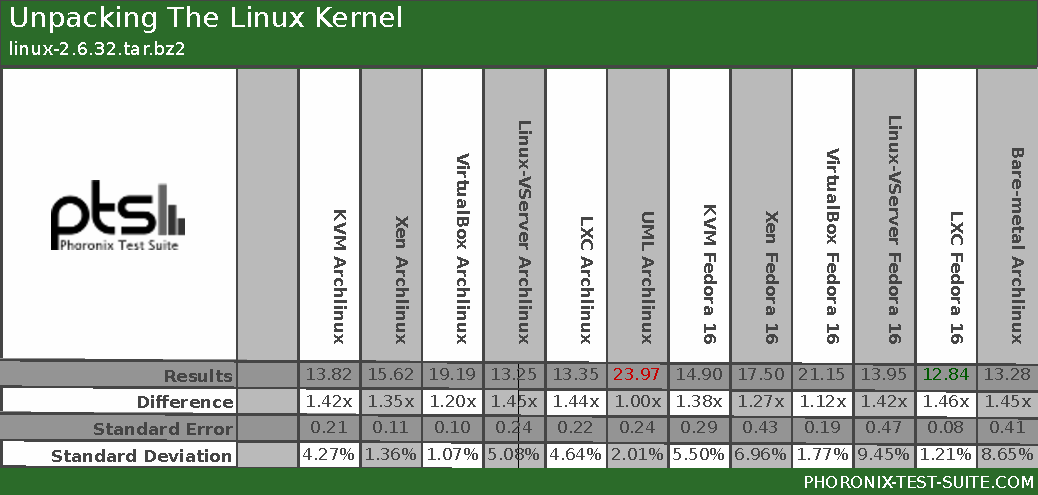
\includegraphics[width=15cm]{obr/bench/unpack-linux-table}
  \caption{Doba za jak dlouho se rozbalí zdrojové kódy jádra linuxu.}
  \label{obr:bench:unpacklinux}
\end{figure}


\begin{figure}[h!]
  \centering
  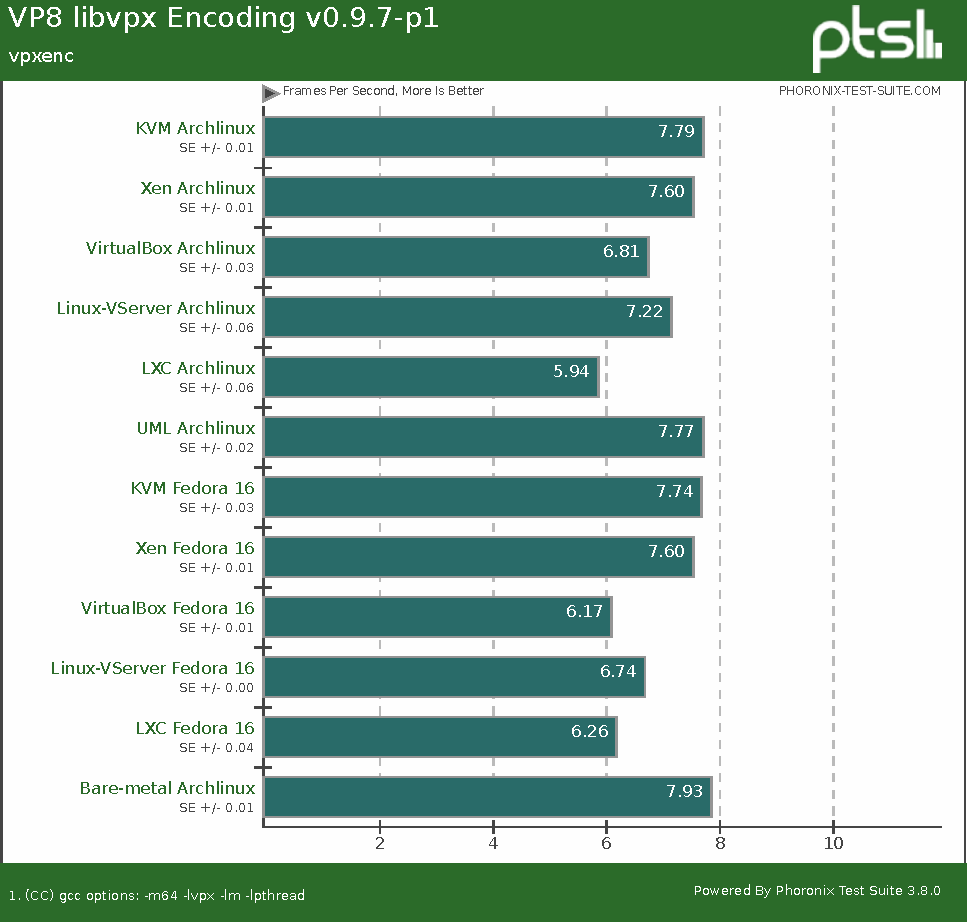
\includegraphics[width=15cm]{obr/bench/vpxenc-graph}
  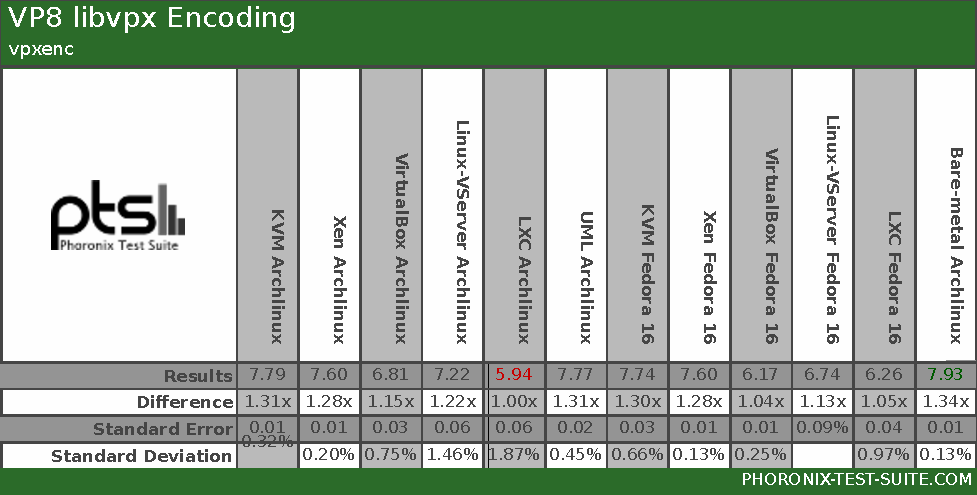
\includegraphics[width=15cm]{obr/bench/vpxenc-table}
  \caption{Počet snímků za sekundu - enkódování do VP8.}
  \label{obr:bench:vpxenc}
\end{figure}



\begin{figure}[h!]
  \centering
  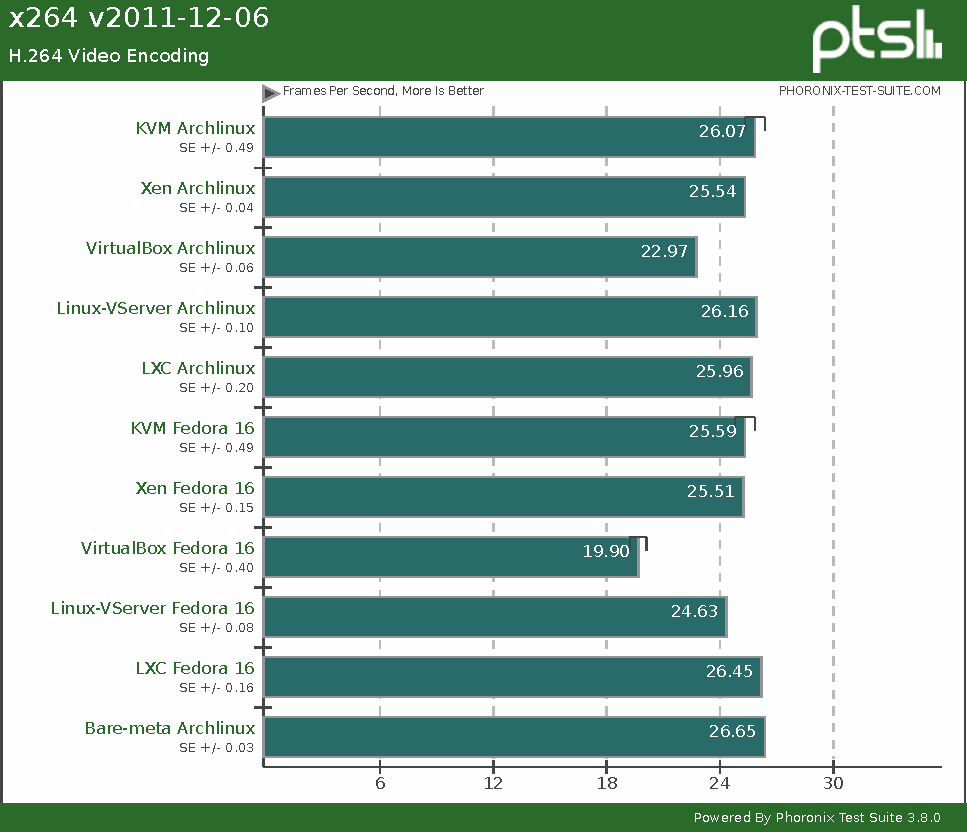
\includegraphics[width=15cm]{obr/bench/x264-graph}
  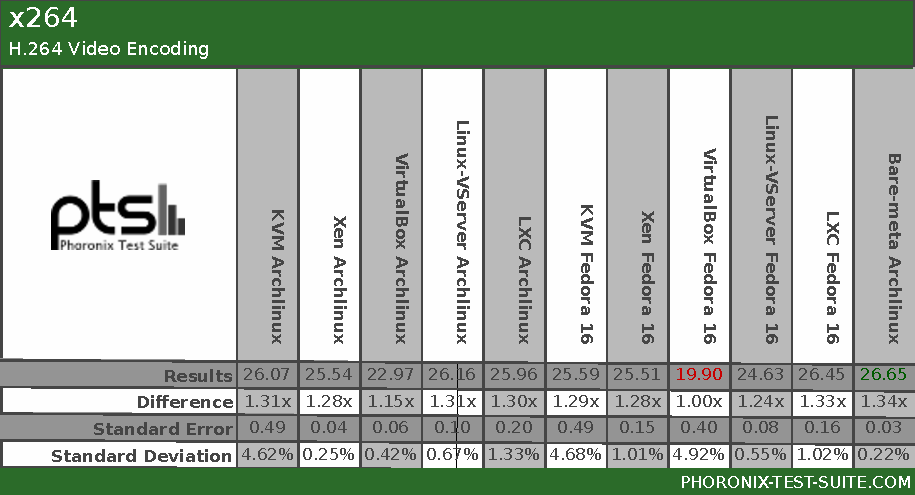
\includegraphics[width=15cm]{obr/bench/x264-table}
  \caption{Počet snímků za sekundu - enkódování do H264.}
  \label{obr:bench:x264}
\end{figure}


\chapter{Závěr}
Všechny nástroje prezentovány v této práci mají určitě svoje využití a nedá se určit jasný vítěz. Velmi totiž záleží právě na účelu pro jaký má být virtualizace použita, co se od ní očekává a co všechno musí umět a podporovat.

Pokud bych měl zhodnotit čistě výkon jednotlivých virtualizačních nástrojů, založený na výsledcích mého testování, tak nejlepšího výkonu bylo dosaženo při použití kontejnerových řešení. A to zejména s distribucí Fedora Core 16 jako hostem. Průměrná režie těchto řešení je pod 5\,\%. Na druhou stranu LXC i Linux-VServer mají svá značná omezení, která plynou z faktu že se nejedná a plnohodnotnou virtualizaci. Tudíž ačkoliv nabízí perfektní výkon a využití zdrojů, nebudou vždy možné použít. Zejména ne tam, kde je primárním cílem izolace a stabilita systému.

V takovém prostředí se spíš vyplatí nasadit některé z plnohodnotných virtualizačních řešení (KVM, Xen nebo VirtualBox). Pokud se podíváme na mé testy, tak zjistíme, že například VirtualBox co se týče výkonu za svými konkurenty pokulhává. Na druhou stranu pokud nám nevadí určitá režie navíc, nabízí nám velmi dobře propracované ovládací rozhraní. Což může být pro hodně lidí velmi důležité. Například v pracovním prostředí, kde potřebuji testovat software na nejrůznějších systémech a konfiguracích, by pro mě snadnost vytvoření a nastavení virtuálního stroje hrála větší roli, než právě výkon.

Na druhou stranu v prostředí, kde bych měl virtualizovaný například webový a databázový server, bych vyžadoval pokud možno co nejlepší výkon. Potom bych měl na výběr buď Xen hypervizor nebo KVM. V testech ve většině případů dosáhlo lepšího skóre řešení využívající KVM. Díky tomu že je součástí jádra je sním i mnohem méně práce při instalaci a konfiguraci. Proto bych jej upřednostnil před Xen hypervizorem.

Na druhou stranu Xen se dá použít i v prostředí, kde hostitel nepodporuje HW virtualizaci. Zde by volba padla určitě právě na Xen, tedy pokud by daný systém byl dostupný v modifikované verzi pro běh pod Xenem. V opačném případě by řešením bylo použít VirtualBox.

V této práci jsem popsal jednotlivé nástroje s jejich kladnými i zápornými vlastnostmi. V jednotlivých testech jsem se snažil zachytit jejich výkonnost a tím poukázat, který nástroj se jak hodí pro určitou činnost. Tato práce by se samozřejmě dala o několik věcí rozšířit.

Například by mohlo být zajímavé provést ty samé testy na odlišném hostiteli. V ideálním případě odlišném nejen například distribucí systému Linux, ale také s rozdílnou HW konfigurací. Ta by mohla obsahovat procesor od firmy Intel, což by nám mohlo dát představu, která z firem má technologii HW podpory virtualizace lépe zvládnutou. Nebo také to, která je v dnešní době lépe implementovaná v současných verzích virtualizačních nástrojů.

Dále by stálo za to, otestovat různé hodnoty konfigurace jádra, jako například hodnota časovače přerušení (toto jsem popravdě zkoušel u Apache benchmark testu na sestavě KVM a Arch Linux, výkon byl zhruba o 10\% lepší). Například u distribuce Fedora se dá časovač nastavit parametrem jádra při spouštění. Což je výhoda, jelikož není potřeba celé jádro znova zkompilovat. I další změny by mohli mít vliv na výkon. Například zkompilování jádra s podporou přímo konkrétní sady instrukcí pro daný procesor, či zkusit místo standardního I/O plánovače CFQ použít plánovač Deadline). Je toho určitě i mnohem víc, ale to by vydalo na celou knihu a pokud bych to měl vše zahrnout do této práce, nevešel bych se do očekávaného rozsahu této práce.

I tak doufám, že pro případného čtenáře byla tato práce přínosem a pomohla mu s rozšířením jeho znalostí o virtualizačních nástrojích nebo si zvolit vhodný virtualizační nástroj pro jeho potřebu. \cite{dike:uml}
\cite{hagen:xen} \cite{huynh:kvm} \cite{kivity:kvm} \cite{romero:vbox} \cite{ruest:virt} \cite{wiki:ovz}

 % viz. obsah.tex

  % Pouzita literatura
  % ----------------------------------------------
\ifczech
  \bibliographystyle{czechiso}
\else 
  \bibliographystyle{plain}
%  \bibliographystyle{alpha}
\fi
  \begin{flushleft}
  \bibliography{literatura} % viz. literatura.bib
  \end{flushleft}
  \appendix
  
  %\chapter{Obsah CD}
%\chapter{Manual}
%\chapter{Konfigrační soubor}
%\chapter{RelaxNG Schéma konfiguračního soboru}
%\chapter{Plakat}

 % viz. prilohy.tex
\end{document}
